\documentclass[11pt,letterpaper]{article}

% ============================================================================
% PACKAGES
% ============================================================================
\usepackage[utf8]{inputenc}
\usepackage[T1]{fontenc}
\usepackage{helvet}
\renewcommand{\familydefault}{\sfdefault}
\usepackage[margin=0.85in, headheight=28pt]{geometry}
\usepackage{graphicx}
\usepackage{xcolor}
\usepackage{tikz}
\usepackage{tcolorbox}
\usepackage{booktabs}
\usepackage{enumitem}
\usepackage{hyperref}
\usepackage{fancyhdr}
\usepackage{titlesec}
\usepackage{multicol}
\usepackage{listings}
\usepackage{upquote}
\usepackage{amsmath,amssymb}
\usepackage{pgfplots}
\usepackage{array}
\usepackage{longtable}

% Ragged-right paragraph columns to prevent word spacing issues
\newcolumntype{L}[1]{>{\raggedright\arraybackslash}p{#1}}

% Increase vertical spacing between table rows for readability
\renewcommand{\arraystretch}{1.4}

\usepackage{colortbl}
\usepackage{pifont}
\usepackage{setspace}
\usepackage{parskip}
\usepackage{caption}
\usepackage{tabularx}

\pgfplotsset{compat=1.18}
\usetikzlibrary{shapes.geometric, arrows.meta, positioning, calc, decorations.pathreplacing, backgrounds, fit, shadows.blur, matrix, patterns, fadings, shadings}

% ============================================================================
% COLOR DEFINITIONS - Scientific Defense Theme (biosecurity/laboratory feel)
% ============================================================================
% Primary: Deep teal - scientific, medical, biosecurity
\definecolor{deepteal}{HTML}{0E4D4D}
\definecolor{scienceteal}{HTML}{3B8C96}
\definecolor{labcyan}{HTML}{5B9A8B}
% Accent: Barrier gold for warnings and highlights
% Standard ETRA header band gold (consistent across all projection reports)
\definecolor{barriergold}{HTML}{B7950B}
\definecolor{shieldamber}{HTML}{C4883A}
% Domain colors
\definecolor{biogreen}{HTML}{4B7F5E}
\definecolor{chemblue}{HTML}{3A6D85}
\definecolor{nukepurple}{HTML}{5B2C6F}
\definecolor{defenseblue}{HTML}{34495E}
% Neutrals
\definecolor{lightgray}{HTML}{F4F6F7}
\definecolor{medgray}{HTML}{BDC3C7}
\definecolor{softslate}{HTML}{5D6D7E}
\definecolor{textdark}{HTML}{1C2833}

% ============================================================================
% HYPERREF SETUP
% ============================================================================
\hypersetup{
  colorlinks=true,
  linkcolor=deepteal,
  urlcolor=scienceteal,
  pdftitle={AI Agents and WMD Proliferation Risk Assessment},
  pdfauthor={Emerging Technology Risk Assessment}
}

% ============================================================================
% SPACING AND TYPOGRAPHY
% ============================================================================
\setstretch{1.15}
\setlength{\parskip}{0.5em}
\setlist{nosep, leftmargin=1.5em, itemsep=0.3em}

% ============================================================================
% PAGE STYLE - Hexagonal molecular pattern (biosecurity theme)
% ============================================================================
\pagestyle{fancy}
\fancyhf{}
\fancyhead[L]{%
  \begin{tikzpicture}[baseline=-0.5ex]
    % Hexagonal pattern (molecular/biosecurity feel) - larger for visibility
    \foreach \i in {0,1,2} {
      \draw[scienceteal, opacity=0.5, line width=0.6pt]
        ({0.15+\i*0.42},0.15) -- ++(60:0.15) -- ++(0:0.15) -- ++(-60:0.15)
        -- ++(-120:0.15) -- ++(180:0.15) -- cycle;
    }
    \fill[barriergold, opacity=0.8] (0.37,0.15) circle (0.06);
  \end{tikzpicture}
  \hspace{0.4em}\textcolor{deepteal}{\textsf{\small ETRA-2026-WMD-001}}%
}
\fancyhead[R]{\textcolor{softslate}{\textsf{\thepage}}}
\fancyfoot[C]{\textcolor{softslate}{\footnotesize\textsf{Emerging Technology Risk Assessment | Biosecurity Policy Research}}}
\renewcommand{\headrulewidth}{0pt}
\renewcommand{\footrulewidth}{0pt}

\fancyheadoffset{0pt}
\setlength{\headheight}{32pt}

% ============================================================================
% SECTION FORMATTING - Scientific defense style with hexagon accents
% ============================================================================
\titleformat{\section}
  {\normalfont\LARGE\bfseries\color{deepteal}}
  {\thesection}{0.8em}{}[\vspace{-0.3em}{\color{scienceteal}\rule{\textwidth}{1.5pt}\hspace{-\textwidth}\color{barriergold}\rule{3cm}{1.5pt}}]
\titleformat{\subsection}
  {\normalfont\Large\bfseries\color{deepteal}}
  {\thesubsection}{0.6em}{}
\titleformat{\subsubsection}
  {\normalfont\large\color{softslate}\bfseries}
  {\thesubsubsection}{0.5em}{}

\titlespacing*{\section}{0pt}{3ex plus 1ex minus .2ex}{2ex plus .2ex}
\titlespacing*{\subsection}{0pt}{2.5ex plus 1ex minus .2ex}{1.5ex plus .2ex}

\setcounter{tocdepth}{2}

% ============================================================================
% TCOLORBOX ENVIRONMENTS - Scientific defense styling
% ============================================================================
\tcbuselibrary{skins,breakable,hooks}

\newtcolorbox{keybox}[1][Key Finding]{
  enhanced, breakable,
  colback=scienceteal!10, colframe=scienceteal,
  colbacktitle=scienceteal, coltitle=white,
  fonttitle=\bfseries\sffamily,
  title={\ding{72}\hspace{0.5em}#1},
  boxrule=0pt, leftrule=4pt, arc=0pt, outer arc=0pt,
  left=12pt, right=12pt, top=8pt, bottom=8pt
}

\newtcolorbox{contextbox}[1][Context]{
  enhanced, breakable,
  colback=biogreen!10, colframe=biogreen,
  colbacktitle=biogreen, coltitle=white,
  fonttitle=\bfseries\sffamily,
  title={\ding{51}\hspace{0.5em}#1},
  boxrule=0pt, leftrule=4pt, arc=0pt, outer arc=0pt,
  left=12pt, right=12pt, top=8pt, bottom=8pt
}

\newtcolorbox{notebox}[1][Note]{
  enhanced, breakable,
  colback=barriergold!12, colframe=barriergold,
  colbacktitle=barriergold, coltitle=white,
  fonttitle=\bfseries\sffamily,
  title={\ding{73}\hspace{0.5em}#1},
  boxrule=0pt, leftrule=4pt, arc=0pt, outer arc=0pt,
  left=12pt, right=12pt, top=8pt, bottom=8pt
}

\newtcolorbox{infobox}[1][Information]{
  enhanced, breakable,
  colback=chemblue!10, colframe=chemblue,
  colbacktitle=chemblue, coltitle=white,
  fonttitle=\bfseries\sffamily,
  title={\ding{73}\hspace{0.5em}#1},
  boxrule=0pt, leftrule=4pt, arc=0pt, outer arc=0pt,
  left=12pt, right=12pt, top=8pt, bottom=8pt
}

\newtcolorbox{defbox}[1][Definition]{
  enhanced, breakable,
  colback=deepteal!8, colframe=deepteal,
  colbacktitle=deepteal, coltitle=white,
  fonttitle=\bfseries\sffamily,
  title={\ding{70}\hspace{0.5em}#1},
  boxrule=0pt, leftrule=4pt, arc=0pt, outer arc=0pt,
  left=12pt, right=12pt, top=8pt, bottom=8pt
}

\newtcolorbox{quotebox}{
  enhanced, breakable,
  colback=lightgray, colframe=scienceteal!50,
  boxrule=0pt, leftrule=4pt, arc=0pt, outer arc=0pt,
  left=12pt, right=12pt, top=8pt, bottom=8pt
}

\newtcolorbox{barrierbox}[1][Barrier Analysis]{
  enhanced, breakable,
  colback=nukepurple!8, colframe=nukepurple,
  colbacktitle=nukepurple, coltitle=white,
  fonttitle=\bfseries\sffamily,
  title={\ding{74}\hspace{0.5em}#1},
  boxrule=0pt, leftrule=4pt, arc=0pt, outer arc=0pt,
  left=12pt, right=12pt, top=8pt, bottom=8pt
}

% ============================================================================
% DOCUMENT
% ============================================================================
\begin{document}

% ============================================================================
% TITLE PAGE - Concentric Defense Barriers Visualization
% ============================================================================
\begin{titlepage}

\begin{tikzpicture}[remember picture, overlay]
  % Background - deep teal gradient
  \fill[deepteal] (current page.north west) rectangle (current page.south east);

  % Hexagonal pattern background (molecular/biosecurity feel)
  \begin{scope}[shift={(current page.center)}, opacity=0.04]
    \foreach \x in {-8,-6.5,...,10} {
      \foreach \y in {-12,-10.5,...,12} {
        \draw[white, line width=0.3pt]
          (\x,\y) -- ++(60:0.5) -- ++(0:0.5) -- ++(-60:0.5)
          -- ++(-120:0.5) -- ++(180:0.5) -- cycle;
      }
    }
  \end{scope}

  % Main visualization - Concentric Defense Barriers (refined)
  \begin{scope}[shift={([xshift=-1.5cm, yshift=3.5cm]current page.center)}]
    % Subtle radial gradient - depth cue from center outward
    \shade[inner color=white, outer color=deepteal, opacity=0.08] (0,0) circle (6.2cm);

    % Outer barrier ring (weakest - eroding) with breach indicators
    \draw[labcyan, opacity=0.3, line width=10pt] (0,0) circle (5.5cm);
    \draw[labcyan, opacity=0.5, line width=2pt, dashed] (0,0) circle (5.5cm);
    % Middle barrier ring (moderate)
    \draw[scienceteal, opacity=0.4, line width=12pt] (0,0) circle (4cm);
    \draw[scienceteal, opacity=0.6, line width=2pt] (0,0) circle (4cm);

    % Inner barrier ring (strong)
    \draw[barriergold, opacity=0.5, line width=14pt] (0,0) circle (2.5cm);
    \draw[barriergold, opacity=0.8, line width=2pt] (0,0) circle (2.5cm);

    % Core - protected zone with glow
    \shade[inner color=barriergold!60, outer color=barriergold!10, opacity=0.3] (0,0) circle (1.5cm);
    \fill[barriergold] (0,0) circle (0.8cm);
    \node[deepteal, font=\fontsize{7}{7}\selectfont\bfseries] at (0,0.12) {DEFENSE};
    \node[deepteal, font=\fontsize{7}{7}\selectfont\bfseries] at (0,-0.18) {IN DEPTH};
  \end{scope}

  % Legend - right side, professional layout
  \begin{scope}[shift={([xshift=5.5cm, yshift=3.5cm]current page.center)}]
    % Legend background
    \fill[black, opacity=0.2, rounded corners=4pt] (-0.3, -2.0) rectangle (4.2, 2.8);

    % Legend title
    \node[white, opacity=0.6, font=\fontsize{7}{7}\selectfont\sffamily, anchor=west] at (0, 2.3) {DEFENSE LAYERS};
    \draw[white, opacity=0.3, line width=0.5pt] (0, 2.0) -- (3.8, 2.0);

    % Outer ring legend item
    \draw[labcyan, opacity=0.6, line width=3pt, dashed] (0.4, 1.3) -- (1.2, 1.3);
    \node[labcyan, font=\fontsize{8}{8}\selectfont\sffamily\bfseries, anchor=west] at (1.5, 1.3) {Information};
    \node[white, opacity=0.7, font=\fontsize{7}{7}\selectfont\sffamily, anchor=west] at (1.5, 0.9) {Barrier};

    % Middle ring legend item
    \draw[scienceteal, opacity=0.7, line width=3pt] (0.4, 0.1) -- (1.2, 0.1);
    \node[scienceteal, font=\fontsize{8}{8}\selectfont\sffamily\bfseries, anchor=west] at (1.5, 0.1) {Physical};
    \node[white, opacity=0.7, font=\fontsize{7}{7}\selectfont\sffamily, anchor=west] at (1.5, -0.3) {Barrier};

    % Inner ring legend item
    \draw[barriergold, opacity=0.8, line width=3pt] (0.4, -1.1) -- (1.2, -1.1);
    \node[barriergold, font=\fontsize{8}{8}\selectfont\sffamily\bfseries, anchor=west] at (1.5, -1.1) {Tacit};
    \node[white, opacity=0.7, font=\fontsize{7}{7}\selectfont\sffamily, anchor=west] at (1.5, -1.5) {Knowledge};
  \end{scope}

  % Document header bar (keeping consistent format)
  \fill[barriergold] ([yshift=-1.5cm]current page.north west) rectangle ([yshift=-2.2cm]current page.north east);
  \node[deepteal, font=\small\bfseries\sffamily] at ([yshift=-1.85cm]current page.north) {PROJECTION REPORT \textbar{} ETRA-2026-WMD-001 \textbar{} FEBRUARY 2026};

  % Title block
  \node[anchor=south west, text width=14cm] at ([xshift=1.5cm, yshift=3cm]current page.south west) {
    {\fontsize{11}{13}\selectfont\color{barriergold}\sffamily EMERGING TECHNOLOGY RISK ASSESSMENT}\\[0.8cm]
    {\fontsize{36}{42}\selectfont\bfseries\color{white}AI Agents and}\\[0.2cm]
    {\fontsize{36}{42}\selectfont\bfseries\color{white}WMD Proliferation}\\[0.2cm]
    {\fontsize{36}{42}\selectfont\bfseries\color{white}Risk}\\[0.6cm]
    {\large\color{medgray}\sffamily A Policy Research Document on Defensive Preparedness}
  };

  % Metadata block
  \node[anchor=south east, text width=6cm, align=right] at ([xshift=-1.5cm, yshift=3cm]current page.south east) {
    \color{medgray}\small\sffamily
    \textbf{Document Type:} Policy Research\\[0.2em]
    \textbf{Time Horizon:} 2025--2030\\[0.2em]
    \textbf{License:} MIT / Unlicense\\[0.2em]
    \textbf{Version:} 2.0
  };

  % Accent line
  \draw[barriergold, line width=2pt] ([xshift=1.5cm, yshift=3cm]current page.south west) -- ([xshift=1.5cm, yshift=10.5cm]current page.south west);

\end{tikzpicture}
\end{titlepage}

% ============================================================================
% ABOUT THIS DOCUMENT
% ============================================================================
\thispagestyle{empty}
\vspace*{0.5cm}

\noindent\begin{tikzpicture}
  \fill[deepteal] (0,0) rectangle (\textwidth, 0.2);
  % Hexagonal accent pattern - larger for visibility
  \foreach \x in {0.4,1.0,...,16.5} {
    \draw[barriergold, opacity=0.7, line width=0.5pt]
      (\x, 0.1) -- ++(60:0.08) -- ++(0:0.08) -- ++(-60:0.08)
      -- ++(-120:0.08) -- ++(180:0.08) -- cycle;
  }
\end{tikzpicture}

\vspace{0.5cm}
\begin{center}
{\color{deepteal}\Large\bfseries About This Document}
\end{center}
\vspace{0.3cm}

\begin{tcolorbox}[enhanced, colback=lightgray, colframe=scienceteal!60, boxrule=1pt, arc=3pt,
  left=10pt, right=10pt, top=10pt, bottom=10pt]
This is a \textbf{public policy research document} analyzing how AI capabilities may affect WMD proliferation risks. It is released under permissive open-source licenses (MIT/Unlicense) to support broad discussion of these governance challenges.

\vspace{0.5em}
\textbf{Independent Work:} This report is independent research. It is not affiliated with, produced by, or endorsed by any government agency, think tank, or official institution. The ``ETRA'' identifier is a document formatting convention, not an organizational identity.
\end{tcolorbox}

\vspace{0.5cm}

\begin{minipage}[t]{0.48\textwidth}
\textbf{Intended Audiences:}
\begin{itemize}[nosep]
  \item Policy researchers and analysts
  \item AI safety and security researchers
  \item Academic communities studying technology governance
  \item Journalists covering AI risks
  \item General public interested in emerging technology policy
\end{itemize}
\end{minipage}
\hfill
\begin{minipage}[t]{0.48\textwidth}
\textbf{How to Use This Document:}
\begin{itemize}[nosep]
  \item The analysis is framed for \textit{defensive} purposes
  \item Technical details that could enable harm are intentionally omitted
  \item Probability estimates are discussion aids, not predictions
  \item When excerpting, please preserve context
\end{itemize}
\end{minipage}

\vspace{0.8cm}

\begin{contextbox}[What This Document Is NOT Claiming]
To prevent misreading, we explicitly clarify:
\begin{itemize}
  \item \textbf{NOT claiming an imminent WMD wave.} Actual WMD attacks by non-state actors remain extremely rare. Our assessment is that \textit{attempt frequency} may increase while \textit{success rate} remains low.
  \item \textbf{NOT claiming novices can build WMD.} AI does not transform a curious novice (T0) into a capable threat actor. The primary effect is upgrading T1--T3 actors who already have partial capability.
  \item \textbf{NOT claiming AI is the dominant proliferation driver.} Geopolitics, state programs, and traditional pathways remain more significant than AI-enabled non-state threats in most scenarios.
  \item \textbf{NOT claiming restriction-only solutions work.} Effective strategy requires balanced investment in detection, attribution, response, and resilience.
  \item \textbf{NOT claiming high confidence in probability estimates.} Scenario probabilities are subjective priors for decision support, not empirical predictions.
\end{itemize}
\end{contextbox}

\vspace{0.5cm}

\begin{infobox}[Epistemic Status Markers]
Throughout this document, key claims are tagged with epistemic status:
\begin{center}
\small
\begin{tabular}{L{1.5cm}L{4cm}L{6cm}}
\toprule
\textbf{Marker} & \textbf{Meaning} & \textbf{Evidence Standard} \\
\midrule
\textbf{[O]} & Open-source documented & Published research, official statements, public data \\
\textbf{[E]} & Expert judgment & Consistent with theory and limited evidence; gaps acknowledged \\
\textbf{[S]} & Speculative projection & Extrapolation from trends; significant uncertainty \\
\bottomrule
\end{tabular}
\end{center}
\end{infobox}

\newpage

% ============================================================================
% EXECUTIVE SUMMARY
% ============================================================================
\section*{Executive Summary}
\addcontentsline{toc}{section}{Executive Summary}

This projection examines how autonomous AI agents may alter the proliferation landscape for weapons of mass destruction (WMD). We analyze current technological capabilities as of early 2026, project scenarios through 2030, and examine the interplay between AI capabilities, existing physical barriers, and potential defensive adaptations.

\begin{keybox}[Key Findings]
\begin{enumerate}
  \item \textbf{[E]} Agentic AI workflows are unlikely to enable a novice (T0) to construct a functional WMD, but they will meaningfully lower barriers for T1--T3 actors who already have partial capability
  \item \textbf{[E]} Biological weapons represent the highest-risk category due to eroding physical barriers and AI's strength in knowledge synthesis
  \item \textbf{[E]} The ``tacit knowledge gap'' remains significant, but AI-guided systems and cloud labs are beginning to erode it
  \item \textbf{[O]} Nuclear weapons face the strongest physical barriers; AI primarily assists state-level (T4) programs
  \item \textbf{[E]} Cyber-physical attacks on existing WMD-adjacent infrastructure (BSL-4 labs, chemical plants) may represent higher near-term risk than de novo synthesis
  \item \textbf{[E]} The ``high-frequency attempts, limited success'' scenario is more likely than catastrophic mass-casualty events; defenders should prepare for resource strain from numerous low-sophistication incidents
\end{enumerate}
\end{keybox}

\subsection*{Why Now? Capability Shift 2023--2026}

\begin{center}
\small
\begin{tabular}{L{3cm}L{4cm}L{4cm}L{2.5cm}}
\toprule
\textbf{Capability} & \textbf{2023 State} & \textbf{2025 State} & \textbf{Impact} \\
\midrule
Agentic autonomy & Chatbots provided info & Agents execute multi-step tasks; delegate to sub-agents \textbf{[O]} & Knowledge $\to$ execution \\
Reasoning models & No explicit chain-of-thought & Dedicated reasoning models (o3, DeepSeek R1) with multi-step planning \textbf{[O]} & Expert-level planning \\
Vision-language & Text-only instruction & Real-time visual interpretation; wearable integration \textbf{[O]} & Bridges tacit knowledge \\
Computer Use & Manual web interaction & Agents browse, fill forms; MCP enables hardware control \textbf{[O]} & Procurement automation \\
Biological design & AlphaFold 2 (structure) & AlphaFold 3, ESM3, Evo, RFdiffusion (generative) \textbf{[O]} & Optimization capability \\
Open-weight models & Limited high-capability & DeepSeek R1/V3, Llama 3.3, Qwen 2.5 with fine-tuning \textbf{[O]} & Guardrail bypass; open reasoning \\
\bottomrule
\end{tabular}
\end{center}

\subsection*{Base-Rate Context: Anchoring Expectations}

\begin{quotebox}
\textbf{Actual WMD attacks by non-state actors remain extremely rare.} The 1995 Tokyo subway attack and 2001 anthrax letters represent essentially the entire modern history of non-state WMD use. The overwhelming majority of WMD-related arrests involve early-stage planning with minimal actual capability.

\textbf{The dominant near-term concern is likely:}
\begin{itemize}[nosep]
  \item Increased frequency of \textit{attempts} with varying degrees of competence
  \item Crude attacks with limited casualties but significant psychological impact
  \item State-level proliferation acceleration using AI assistance
  \item Erosion of verification regimes as AI complicates attribution
\end{itemize}

Readers should interpret this analysis through that lens: the primary concern is \textit{barrier reduction enabling more attempts}, with catastrophic mass-casualty events remaining low-probability tail risks.
\end{quotebox}

\newpage
\tableofcontents
\newpage

% ============================================================================
% ONE-PAGE EXECUTIVE SUMMARY
% ============================================================================
\section*{Quick Reference: One-Page Summary}
\addcontentsline{toc}{section}{Quick Reference: One-Page Summary}

\subsection*{Core Claims}

\begin{enumerate}
  \item \textbf{Biological weapons are the highest-risk category} for AI-enabled proliferation due to eroding physical barriers and high AI contribution to knowledge synthesis
  \item \textbf{AI primarily upgrades T1--T3 actors} (skilled individuals to organized groups); it does not transform novices into capable threat actors
  \item \textbf{The most likely near-term scenario is high-frequency attempts with limited success}---resource strain and public concern, not mass casualties
  \item \textbf{Cyber-physical attacks on existing infrastructure} (labs, chemical plants) may be higher-leverage than synthesis assistance
  \item \textbf{Governance windows are closing}---once capabilities proliferate, restrictions become harder to implement
\end{enumerate}

\subsection*{Top 5 Recommended Actions}

\begin{enumerate}
  \item \textbf{Mandate universal DNA synthesis screening} with international harmonization
  \item \textbf{Invest in attribution and response capabilities}---cannot rely on deterrence alone
  \item \textbf{Establish cloud laboratory oversight frameworks} before the attack surface expands further
  \item \textbf{Require WMD-relevant capability evaluations} before frontier AI deployment
  \item \textbf{Fund defensive biodetection} as a high-value cross-threat investment
\end{enumerate}

\subsection*{Top 5 Indicators to Monitor}

\begin{enumerate}
  \item DNA synthesis screening intercept rates and patterns
  \item AI model performance on biology/chemistry benchmarks
  \item Cloud laboratory service expansion and security posture
  \item Dark web discussion of AI + WMD capabilities
  \item Progress (or lack thereof) on international governance coordination
\end{enumerate}

\subsection*{What Would Change This Assessment}

\begin{minipage}[t]{0.48\textwidth}
\textbf{Would Increase Concern:}
\begin{itemize}[nosep]
  \item Confirmed AI-assisted WMD attempt
  \item Release of unrestricted biology-capable research agent
  \item Major cloud lab security breach
\end{itemize}
\end{minipage}
\hfill
\begin{minipage}[t]{0.48\textwidth}
\textbf{Would Decrease Concern:}
\begin{itemize}[nosep]
  \item Effective international AI safety framework
  \item Robust attribution breakthrough
  \item AI guardrails prove more durable than expected
\end{itemize}
\end{minipage}

\subsection*{Reading Guide}

This document is comprehensive. For targeted reading based on role:

\begin{center}
\small
\begin{tabular}{L{3.5cm}L{7cm}L{1.5cm}}
\toprule
\textbf{Reader Profile} & \textbf{Recommended Sections} & \textbf{Time} \\
\midrule
Policymaker / Executive & Executive Summary + Policy Recommendations + Scenarios & $\sim$20 min \\
Security Practitioner & Deployment Vectors + Cyber-Physical + Attribution + Signals & $\sim$25 min \\
AI Safety Researcher & Methodology + Frameworks + Technology + Counterarguments & $\sim$30 min \\
Biosecurity Specialist & Biological Weapons + Gene Drives + Companion Research + Policy & $\sim$20 min \\
General Reader & One-Page Summary + Counterarguments + Civil Liberties + Conclusion & $\sim$15 min \\
\bottomrule
\end{tabular}
\end{center}

\subsection*{Related ETRA Reports}

This projection is part of a series of Emerging Technology Risk Assessment reports. Several contain analysis directly relevant to WMD proliferation:

\begin{center}
\small
\begin{tabular}{L{5cm}L{7cm}}
\toprule
\textbf{Report} & \textbf{Key WMD-Relevant Concepts} \\
\midrule
AI Agents and Espionage Operations & ``Democratization of tradecraft'' parallels WMD barrier reduction; offense-defense timeline \\
AI Agents and Financial Integrity & ``Nano-smurfing'' maps to procurement evasion; ``weakest-link exploitation'' in export controls \\
AI Agents and Institutional Erosion & IC capacity degradation weakens proliferation monitoring; ``Delegation Defense'' complicates attribution \\
AI Agents and Political Targeting & Power Diffusion Theory as shared framework; ``conspiracy footprint shrinks'' \\
\bottomrule
\end{tabular}
\end{center}

\newpage

% ============================================================================
% PART I - FOUNDATIONS
% ============================================================================
\clearpage
\thispagestyle{empty}
\vspace*{-0.85in}
\noindent\hspace*{-0.85in}\begin{tikzpicture}
  \fill[deepteal] (0,0) rectangle (\paperwidth, -10cm);

  \node[barriergold, font=\fontsize{10}{10}\selectfont\sffamily] at (0.5\paperwidth, -1.2cm) {PART I};
  \node[white, font=\fontsize{48}{48}\selectfont\bfseries] at (0.5\paperwidth, -2.8cm) {Foundations};
  \node[white, opacity=0.7, font=\normalsize\sffamily] at (0.5\paperwidth, -4.2cm) {Theory, Capabilities, and Historical Context};

  % Interlocking gears visualization - centered above gold line
  \begin{scope}[shift={(0.5\paperwidth, -7cm)}]
    % Subtle background panel
    \fill[black, opacity=0.15, rounded corners=3pt] (-5.0, -2.0) rectangle (5.0, 2.0);

    % Gear tooth style
    \tikzset{
      gear tooth/.style={line width=2pt, line cap=round}
    }

    % Left gear - Theory (medium, 8 teeth)
    \begin{scope}[shift={(-2.4, 0.3)}]
      \fill[scienceteal, opacity=0.6] (0,0) circle (1.15cm);
      \fill[scienceteal, opacity=0.8] (0,0) circle (0.95cm);
      % Gear teeth
      \foreach \angle in {0, 45, 90, 135, 180, 225, 270, 315} {
        \fill[scienceteal, opacity=0.8] (\angle:0.95cm) -- (\angle+12:1.35cm) -- (\angle-12:1.35cm) -- cycle;
      }
      \fill[deepteal, opacity=0.9] (0,0) circle (0.6cm);
      \node[scienceteal, font=\fontsize{6}{6}\selectfont\sffamily\bfseries] at (0, 0) {THEORY};
    \end{scope}

    % Center gear - Capabilities (large, 10 teeth) - main driver
    \begin{scope}[shift={(0.4, -0.5)}]
      \fill[barriergold, opacity=0.5] (0,0) circle (1.45cm);
      \fill[barriergold, opacity=0.7] (0,0) circle (1.25cm);
      % Gear teeth
      \foreach \angle in {0, 36, 72, 108, 144, 180, 216, 252, 288, 324} {
        \fill[barriergold, opacity=0.8] (\angle:1.25cm) -- (\angle+10:1.65cm) -- (\angle-10:1.65cm) -- cycle;
      }
      \fill[deepteal, opacity=0.95] (0,0) circle (0.9cm);
      \node[barriergold, font=\fontsize{6}{6}\selectfont\sffamily\bfseries] at (0, 0) {CAPABILITIES};
    \end{scope}

    % Right gear - Context (medium, 8 teeth)
    \begin{scope}[shift={(3.2, 0.6)}]
      \fill[labcyan, opacity=0.5] (0,0) circle (1.1cm);
      \fill[labcyan, opacity=0.7] (0,0) circle (0.9cm);
      % Gear teeth
      \foreach \angle in {0, 45, 90, 135, 180, 225, 270, 315} {
        \fill[labcyan, opacity=0.8] (\angle:0.9cm) -- (\angle+12:1.3cm) -- (\angle-12:1.3cm) -- cycle;
      }
      \fill[deepteal, opacity=0.9] (0,0) circle (0.55cm);
      \node[labcyan, font=\fontsize{6}{6}\selectfont\sffamily\bfseries] at (0, 0) {CONTEXT};
    \end{scope}
  \end{scope}

  \fill[barriergold] (2cm, -9.2cm) rectangle (\paperwidth-2cm, -9.3cm);
\end{tikzpicture}

\vspace{0.8cm}

\section{Introduction and Methodology}

\subsection{Purpose}

The development of weapons of mass destruction has historically required either state-level resources or exceptional individual expertise. The Manhattan Project employed over 125,000 people. Aum Shinrikyo, despite millions of dollars and multiple PhD scientists, failed to effectively weaponize biological agents.

We are now entering an era where autonomous AI agents capable of complex multi-step planning become widely accessible. This projection examines whether and how AI agents might erode these historical barriers.

\textbf{Critical framing}: This analysis does not assume WMD attacks will increase. The goal is to understand how AI capabilities change the \textit{nature} of proliferation risks, identify which categories face the greatest barrier reduction, and recommend defensive preparations.

\subsection{Methodology}

This analysis draws on:
\begin{itemize}
  \item \textbf{Current capability assessment} of AI systems and synthetic biology tools as deployed through early 2026
  \item \textbf{Historical case analysis} of WMD development programs (state and non-state)
  \item \textbf{Dual-Use Research of Concern (DURC)} literature and policy debates
  \item \textbf{Expert consultation} across biosecurity, nuclear security, and AI safety domains
  \item \textbf{Red team exercises} examining potential applications (conducted under controlled conditions)
\end{itemize}

We deliberately avoid: specific technical implementation details, named pathogen sequences or synthesis routes, and information not already publicly available in academic literature.

\subsection{What We've Observed in 2025}

Evidence regarding AI-assisted biosecurity threats, categorized by epistemic status:

\textbf{Demonstrated in open evaluations:}
\begin{itemize}[nosep]
  \item AI models can provide general information about pathogen biology from open literature
  \item Frontier AI models refuse most explicit requests for weapons guidance but inconsistencies exist
  \item AI systems show measurable ``uplift'' in non-expert comprehension of complex biological concepts
\end{itemize}

\textbf{Supported by limited disclosures:}
\begin{itemize}[nosep]
  \item DNA synthesis screening has intercepted concerning orders (industry statements, limited specifics)
  \item Security services have begun integrating AI into threat monitoring
\end{itemize}

\textbf{Speculative / emerging:}
\begin{itemize}[nosep]
  \item AI-enabled gain-of-function design assistance (theoretical capability, no documented attempts)
  \item Cloud laboratory exploitation for harmful protocols (no known incidents)
\end{itemize}

\textbf{Absence of evidence (notable):}
\begin{itemize}[nosep]
  \item No documented cases of AI-enabled biological weapon development
  \item No confirmed AI-assisted WMD attacks or advanced attempts
\end{itemize}

\subsection{Definitions}

\begin{defbox}[Core Definitions]
\textbf{Chatbot vs. Autonomous Research Agent} (critical 2025 distinction):

\vspace{0.5em}
\begin{center}
\small
\begin{tabular}{L{3cm}L{5cm}L{4cm}}
\toprule
\textbf{Type} & \textbf{Capability} & \textbf{Risk Profile} \\
\midrule
Chatbot (2022--23) & Provides information; no tool use; no persistence & Knowledge aggregation only \\
Autonomous Agent (2024--25) & Multi-step tasks; tools; self-correction; context persistence & Shifts knowledge to execution \\
Reasoning Agent (2025--26) & Dedicated chain-of-thought reasoning; multi-step planning; sub-agent delegation & Expert-level planning and optimization; multi-agent orchestration \\
\bottomrule
\end{tabular}
\end{center}

\vspace{0.5em}
\textbf{Biological Design Tools (BDTs)}: Specialized AI models for biological research (AlphaFold 3, ESM3, RFdiffusion). Often fewer guardrails than consumer chatbots.

\vspace{0.5em}
\textbf{Computer Use Capabilities}: AI agents interacting with GUIs, browsing, filling forms (Claude computer use, OpenAI Operator). Enables autonomous procurement.

\vspace{0.5em}
\textbf{Uplift}: The degree to which AI assistance improves a non-expert's ability to accomplish a dangerous task.
\end{defbox}

\subsection{AI Agent Capabilities}

AI agents in early 2026 can:
\begin{itemize}[nosep]
  \item Synthesize information from thousands of scientific papers in seconds
  \item Conduct extended multi-step research tasks with minimal supervision
  \item Operate tools including web browsers, code execution, and API interactions
  \item Interface with laboratory information management systems (LIMS) and laboratory hardware via protocols such as MCP
  \item Generate and optimize experimental protocols
  \item Analyze results and iteratively refine approaches
  \item Maintain persistent goals across sessions
  \item Delegate sub-tasks to specialized sub-agents, enabling multi-agent workflows
  \item Perform extended chain-of-thought reasoning for complex planning tasks (reasoning models)
\end{itemize}

\subsection{Threat Actor Taxonomy}

To avoid the misleading implication that ``AI democratizes WMD to everyone,'' this report uses a tiered actor model:

\begin{center}
\small
\begin{tabular}{L{1cm}L{3.5cm}L{3.5cm}L{4cm}}
\toprule
\textbf{Tier} & \textbf{Description} & \textbf{Pre-AI Capability} & \textbf{Examples} \\
\midrule
T0 & Curious novice & No practical capability & Online researchers \\
T1 & Skilled individual with access & Limited by knowledge gaps & Disgruntled lab worker \\
T2 & Small funded group & Constrained by coordination & Extremist cell \\
T3 & Organized non-state & Historically capable (Aum) & Terrorist organizations \\
T4 & State or state-backed & Full WMD capability & Nation-state programs \\
\bottomrule
\end{tabular}
\end{center}

\textbf{Key insight}: AI primarily benefits T1--T3 actors by reducing knowledge aggregation barriers---it does not transform T0 into T3.

\subsection{Synthetic Biology Infrastructure (2025)}

The infrastructure for synthetic biology has expanded dramatically, creating new touchpoints for both legitimate research and potential misuse:

\textbf{DNA Synthesis Services}:
\begin{itemize}[nosep]
  \item Multiple commercial providers offer gene synthesis with turnaround in days
  \item Costs have dropped to cents per base pair
  \item International providers vary in screening rigor
\end{itemize}

\textbf{Cloud Laboratory Services}:
\begin{itemize}[nosep]
  \item Commercial platforms offer remote access to automated wet labs via API
  \item Equipment includes liquid handlers, PCR machines, sequencers
  \item Geographic distribution creates regulatory arbitrage opportunities
\end{itemize}

\textbf{Open-Source Tools}:
\begin{itemize}[nosep]
  \item Bioinformatics toolkits freely available (Biopython, NCBI tools)
  \item CRISPR design tools accessible to non-experts
  \item Protocols shared through platforms like protocols.io
\end{itemize}

\subsection{Current Safeguards}

Existing control regimes face increasing pressure from technological change:

\textbf{DNA Synthesis Screening}:
\begin{itemize}[nosep]
  \item IGSC (International Gene Synthesis Consortium) guidelines screen against known pathogen sequences
  \item Novel or chimeric sequences may evade detection
  \item Not all providers are IGSC members
  \item Benchtop synthesizers bypass commercial screening entirely
\end{itemize}

\textbf{Export Controls}:
\begin{itemize}[nosep]
  \item Australia Group guidelines cover dual-use equipment
  \item National implementation varies significantly
  \item Dual-use nature of equipment makes enforcement challenging
  \item Digital information largely uncontrolled
\end{itemize}

\textbf{Institutional Biosafety}:
\begin{itemize}[nosep]
  \item Institutional Biosafety Committees (IBCs) review research at formal institutions
  \item Select Agent regulations govern most dangerous pathogens
  \item Gaps exist for independent researchers and DIY biology spaces
  \item International variation in biosafety standards
\end{itemize}

\subsection{Vision-Language Models and Tacit Knowledge Erosion}

The traditional ``tacit knowledge'' barrier assumed that laboratory skills require hands-on training. Vision-Language Models (VLMs) that can ``see'' through cameras are beginning to erode this barrier.

\begin{center}
\small
\begin{tabular}{L{3.5cm}L{4cm}L{4.5cm}}
\toprule
\textbf{VLM Generation} & \textbf{Capability} & \textbf{Tacit Knowledge Impact} \\
\midrule
Text-only LLMs (2022--23) & Written instruction only & Cannot interpret physical observations \\
Basic VLMs (2024) & Static image interpretation & Can identify equipment, reagents \\
Advanced VLMs (2025) & Real-time video analysis & Can provide feedback on ongoing procedures \\
Projected (2026+) & Integrated lab automation & Direct control of robotic systems \\
\bottomrule
\end{tabular}
\end{center}

\textbf{Visual Troubleshooting Scenario} (for defender awareness): Smart glasses can stream video to cloud VLMs \textbf{[O]}. An actor could receive real-time audio feedback while performing procedures. VLM interprets visual state (``color too dark,'' ``precipitate forming'') and suggests adjustments \textbf{[E]}. This partially substitutes for the mentor-mentee relationship that traditionally transmitted tacit knowledge.

\textbf{Current limitation} \textbf{[E]}: VLMs still make errors on domain-specific interpretation; a failed procedure may be unrecoverable. But the gap is narrowing with each model generation.

\subsection{Multi-Agent Delegation and Tool-Use Protocols}

Modern AI agent frameworks increasingly support multi-agent delegation, where a ``supervisor'' agent decomposes a complex task and delegates sub-tasks to specialized ``worker'' agents. This creates a qualitatively different risk profile from single-agent systems.

\textbf{The multi-agent risk}:
\begin{itemize}[nosep]
  \item No single agent sees the complete picture of a harmful workflow
  \item Per-model safety guardrails may not trigger because each sub-task appears innocuous in isolation
  \item Example: Agent A researches pathogen biology (legitimate query); Agent B optimizes a synthesis protocol (legitimate chemistry); Agent C coordinates procurement (legitimate commerce)---no individual agent processes a ``build a weapon'' request, but the orchestrating system assembles the pieces
\end{itemize}

\textbf{Tool-use protocols (MCP and similar)} \textbf{[O]}: The Model Context Protocol (MCP) and similar frameworks enable AI agents to directly interact with external tools: laboratory equipment, procurement platforms, and hardware control systems. This moves agents beyond web browsing and code execution to \textit{physical actuation}---a qualitative shift from information provision to real-world effect.

\textbf{Actor tier relevance}: Multi-agent orchestration primarily benefits T2--T3 actors with technical sophistication. However, as ``agent-as-a-service'' platforms emerge, the barrier is dropping toward T1.

\subsection{Reasoning Models and Complex Planning}

Dedicated reasoning models (o3/o4-mini, Claude extended thinking, DeepSeek R1) represent a step change in AI planning capability \textbf{[O]}. Unlike standard language models, reasoning models perform extended internal chain-of-thought before producing output.

\textbf{The agentic loop amplifier}: The combination of reasoning models with agentic tool use creates a particularly significant capability shift:
\begin{enumerate}[nosep]
  \item \textbf{Plan}: Decompose a complex goal into executable steps with explicit chain-of-thought
  \item \textbf{Execute}: Use tools to carry out each step
  \item \textbf{Observe}: Analyze the results of execution
  \item \textbf{Adjust}: Revise the plan based on observed outcomes
  \item \textbf{Retry}: Iterate without human intervention until the goal is achieved
\end{enumerate}

This ``agentic loop'' is qualitatively different from single-query chatbot interaction. Where a chatbot provides one-shot information, an agentic reasoning system can \textit{iterate through failures autonomously}---the same adaptive learning that makes human experts effective, now operating at machine speed.

\textbf{Current limitation} \textbf{[E]}: As of early 2026, reasoning models excel at well-defined planning tasks but remain unreliable for novel physical procedures where ground-truth feedback is ambiguous.

\textbf{Actor tier relevance}: Reasoning models are widely available (including open-weight: DeepSeek R1). They primarily benefit T1--T3 actors by providing systematic, multi-step planning that previously required expert-level domain knowledge.

\subsection{Governance Challenge: Open-Weight Models}

Most AI safety measures exist at the API level for closed commercial models. Open-weight models present a distinct governance challenge:

\begin{center}
\small
\begin{tabular}{L{3cm}L{2cm}L{2cm}L{2cm}L{3cm}}
\toprule
\textbf{Model Type} & \textbf{Guardrails} & \textbf{Monitoring} & \textbf{Fine-tuning} & \textbf{Governance Lever} \\
\midrule
Closed API (GPT-4.5, Claude 4.5) & Strong & Yes & No & Provider responsibility \\
Open-weight general (Llama 3.3, Qwen 2.5) & Varies & No (local) & Yes & Release decisions only \\
Open-weight reasoning (DeepSeek R1) & Often minimal & No (local) & Yes & Extremely difficult \\
Fine-tuned variants & Often removed & No & Already done & Difficult to control \\
Specialized biology (Evo, domain) & May be absent & No & Domain-specific & Research community norms \\
\bottomrule
\end{tabular}
\end{center}

\textbf{Policy implications}: (1) Pre-release capability evaluation, (2) Compute governance as monitoring opportunity, (3) Community norms on responsible release, (4) Accept that some proliferation is unavoidable---invest in detection accordingly.

\section{Theoretical Frameworks}

This analysis draws on several established theoretical frameworks from security studies, biosecurity, and technology policy.

\subsection{The Democratization of Lethality}

\textbf{Audrey Kurth Cronin's framework} from ``Power to the People'' (2020) describes how each technological era redistributes the capacity for violence. AI represents the latest such redistribution, but with a crucial difference: previous technologies (dynamite, small arms) democratized \textit{physical} capabilities. AI democratizes \textit{cognitive} capabilities---the planning, knowledge synthesis, and optimization that previously required years of specialized training.

For WMD, this means:
\begin{itemize}[nosep]
  \item The barrier was never purely physical (materials exist)
  \item The barrier was also cognitive (knowing what to do with materials)
  \item AI specifically attacks the cognitive barrier while physical barriers remain
\end{itemize}

\subsection{Dual-Use Research of Concern (DURC)}

The \textbf{DURC framework}, developed through debates over H5N1 transmissibility research (2011--2012), recognizes that legitimate scientific research can generate knowledge applicable to harmful purposes. Key insights:
\begin{itemize}[nosep]
  \item Information cannot be ``un-discovered''
  \item Publication decisions involve weighing scientific benefit against misuse potential
  \item The research community has historically self-regulated through institutional review
\end{itemize}

AI agents challenge this framework because they can synthesize DURC-relevant information from dispersed, individually innocuous sources; publication decisions become moot when AI can reconstruct restricted information; and self-regulation assumes human researchers as the primary actors.

\subsection{Information Hazards Framework}

\textbf{Nick Bostrom's concept of ``information hazards''} identifies categories of knowledge that, once disseminated, can cause harm regardless of intent:
\begin{itemize}[nosep]
  \item \textbf{Data hazards}: Specific information enabling harmful actions (pathogen sequences, synthesis routes)
  \item \textbf{Idea hazards}: Concepts that suggest new harmful possibilities
  \item \textbf{Attention hazards}: Drawing attention to vulnerabilities
\end{itemize}

AI agents challenge information hazard management because they can reconstruct restricted information from dispersed innocuous sources, lower the barrier from ``knowledge'' to ``actionable guidance,'' and personalize dangerous information to specific user capabilities.

\subsection{The Unilateralist's Curse}

\textbf{Bostrom and Ord's ``Unilateralist's Curse''} describes a critical dynamic: when a capability becomes accessible to many actors, even if the vast majority (99.9\%) are responsible, the small minority (0.1\%) who would misuse it will eventually do so.

For AI and WMD: AI democratizes access to planning and synthesis knowledge; as millions gain access, the ``curse'' becomes statistically inevitable; the question shifts from ``whether'' to ``when'' and ``how catastrophic''; and defensive strategies must assume misuse will be attempted.

\subsection{Unified Risk Model}

\begin{center}
\fbox{\parbox{0.85\textwidth}{
\centering
\textbf{Risk = Capability $\times$ Access $\times$ Intent $\times$ Execution $\times$ (1 $-$ Interdiction) $\times$ Impact}
}}
\end{center}

\begin{center}
\small
\begin{tabular}{L{3cm}L{3.5cm}L{2.5cm}L{2.5cm}}
\toprule
\textbf{Factor} & \textbf{AI Contribution} & \textbf{Bio (2025--30)} & \textbf{Nuke (2025--30)} \\
\midrule
Capability (can attempt) & HIGH (knowledge synthesis) & Rising & Stable \\
Access (materials/tools) & MEDIUM (cloud labs) & Rising & Stable (fissile) \\
Intent (motivation) & NONE (AI doesn't create) & Stable & Stable \\
Execution (attempt success) & MEDIUM (guidance) & Rising slowly & Stable \\
Interdiction (detection) & MIXED (both sides) & Declining pressure & Stable (strong) \\
\bottomrule
\end{tabular}
\end{center}

\textbf{Key insight}: AI primarily affects Capability and Access (cognitive barriers). Physical barriers, Intent, and Impact Scale are largely AI-independent.

\subsection{The Tacit Knowledge Gap}

\textbf{Michael Polanyi's concept of tacit knowledge}---skills that cannot be fully articulated and must be learned through practice---is central to understanding WMD barriers. Much of weapons development relies on sensory cues, equipment calibration, and ``laboratory intuition'' accumulated over years.

AI agents can transmit explicit knowledge but traditionally cannot transfer tacit knowledge. However, two developments challenge this:
\begin{enumerate}
  \item \textbf{AI-guided instruction}: Real-time guidance that interprets user observations
  \item \textbf{Cloud laboratories}: Robotic systems that embody tacit knowledge in automated protocols
\end{enumerate}

\subsection{Offense-Defense Balance}

\begin{center}
\small
\begin{tabular}{L{4cm}L{4cm}L{4cm}}
\toprule
\textbf{Factor} & \textbf{Favors Offense} & \textbf{Favors Defense} \\
\midrule
Knowledge accessibility & AI aggregates dispersed information & AI can detect dangerous queries \\
Physical materials & Some barriers eroding (DNA synthesis) & Nuclear/chemical materials controlled \\
Attribution & AI complicates attribution & AI forensics improving \\
Detection & Novel agents may evade detection & AI-enhanced surveillance possible \\
\bottomrule
\end{tabular}
\end{center}

The balance varies significantly across WMD categories, which is why biological, chemical, and nuclear require separate analysis.

\subsection{Key Literature}

\begin{center}
\small
\begin{tabular}{L{4.5cm}L{3.5cm}L{4cm}}
\toprule
\textbf{Work} & \textbf{Author(s)} & \textbf{Relevance} \\
\midrule
\textit{Power to the People} & Cronin (2020) & Technology diffusion and non-state violence \\
\textit{Biohazard} & Alibek (1999) & Soviet bioweapons program; scale of state capabilities \\
\textit{Germs} & Miller, Engelberg, Broad (2001) & History of biological weapons programs \\
\textit{Nuclear Terrorism} & Allison (2004) & Non-state nuclear threats assessment \\
\textit{Personal Knowledge} & Polanyi (1958) & Tacit knowledge theory \\
\textit{NIST AI RMF} & NIST (2023) & AI risk management framework \\
\textit{Information Hazards} & Bostrom (2011) & Framework for dangerous knowledge \\
\textit{The Unilateralist's Curse} & Bostrom \& Ord (2015) & Why misuse becomes inevitable \\
\textit{Countdown to Zero Day} & Zetter (2014) & Stuxnet and cyber-physical attacks \\
\textit{The Demon in the Freezer} & Preston (2002) & Smallpox and bioweapons policy \\
\textit{Destined for War} & Allison (2017) & Great power dynamics \\
\textit{RAND Operational Risks} & RAND (2024) & Definitive uplift study \textbf{[O]} \\
\bottomrule
\end{tabular}
\end{center}

\subsection{2024--2026 Policy Developments}

\begin{center}
\small
\begin{tabular}{L{4cm}L{2cm}L{6cm}}
\toprule
\textbf{Reference} & \textbf{Date} & \textbf{Relevance} \\
\midrule
Bletchley Declaration & Nov 2023 & First international consensus on AI risks including CBRN \textbf{[O]} \\
Seoul AI Safety Summit & May 2024 & Extended Bletchley with specific bio-risk language \textbf{[O]} \\
US Executive Order 14110 & Oct 2023; revoked Jan 2025 & Mandates evaluation of AI role in CBRN threats \textbf{[O]} \\
RAND ``Operational Risks'' & 2024 & Definitive uplift study finding limited current risk \textbf{[O]} \\
Anthropic RSP Framework & 2023--24 & Responsible Scaling Policy with CBRN thresholds \textbf{[O]} \\
OpenAI o1 Biological Uplift Evaluations & 2024 & Reasoning model uplift tests; found modest but measurable uplift \textbf{[O]} \\
EU AI Act Implementation & Aug 2025 & First comprehensive AI regulation; high-risk system requirements \textbf{[O]} \\
EO 14110 Revocation & Jan 2025 & US rescinded prior AI safety order; shifts to industry self-governance \textbf{[O]} \\
DeepSeek R1 Open Release & Jan 2025 & Open-weight reasoning model matching frontier performance \textbf{[O]} \\
\bottomrule
\end{tabular}
\end{center}

\section{Historical Context}

\subsection{State Programs: The Scale of Serious Capability}

\textbf{The Manhattan Project (1942--1945)}: Peak employment 125,000+ workers; cost \$2 billion (\$28 billion in 2025 dollars); required industrial-scale facilities.

\textbf{Soviet Biopreparat Program (1970s--1990s)}: Employed 60,000+ people at peak; dozens of facilities; required decades to develop sophisticated delivery.

\textbf{Key insight}: State-level programs achieved capabilities far beyond what any non-state actor has approached.

\subsection{Non-State Attempts: The Capability Gap}

\textbf{Aum Shinrikyo (1984--1995)}:
\begin{itemize}[nosep]
  \item Resources: \$300 million to \$1 billion
  \item Personnel: Multiple PhD scientists
  \item Biological program: Complete failure
  \item Chemical attack: 13 deaths (far below ambitions)
\end{itemize}

\textbf{Critical lesson}: Despite exceptional resources and expertise, Aum's biological program failed completely. Their chemical attack succeeded but at far lower casualty levels than their ambitions. The gap between \textit{intent and capability} was enormous.

\textbf{Why did Aum fail at bioweapons?}
\begin{enumerate}[nosep]
  \item Tacit knowledge gaps despite theoretical expertise
  \item Difficulty obtaining virulent pathogen strains
  \item Weaponization challenges (delivery systems, stability)
  \item Operational security compromises
\end{enumerate}

\textbf{2001 Anthrax Letters}: Perpetrator likely single individual with professional laboratory access. Outcome: 5 deaths, 17 infections, massive societal disruption. Method: Existing laboratory stocks, not de novo synthesis. \textbf{Critical factor}: \textit{Access} to prepared materials, not synthesis capability.

\textbf{Rajneeshee Bioterror Attack (1984)}: Religious cult in Oregon used \textit{Salmonella typhimurium} (common food pathogen) to contaminate restaurant salad bars. Outcome: 751 illnesses, no deaths, significant disruption. \textbf{Critical lesson}: Low-tech attacks with common agents can achieve ``mass disruption'' without ``mass destruction.'' AI agents could optimize logistics of such simple attacks for massive scale.

\textbf{Stuxnet (2010)}: Nation-state attack (US/Israel) targeting Iranian nuclear centrifuges. Malware caused physical destruction via control system manipulation. Outcome: Significant delay to Iranian nuclear program. \textbf{Critical lesson}: Code can cause physical destruction. This establishes the precedent for ``cyber-physical'' attacks on WMD-related infrastructure---a vector AI agents could enable.

\subsection{Technology Inflection Points}

\begin{center}
\small
\begin{tabular}{L{3.5cm}L{4cm}L{4.5cm}}
\toprule
\textbf{Technology} & \textbf{Effect on Barriers} & \textbf{Limiting Factor} \\
\midrule
Internet (1990s) & Info more accessible & Still required physical capability \\
Genome sequencing (2000s) & Sequences publicly available & Still required synthesis capability \\
CRISPR (2012+) & Gene editing simplified & Still required laboratory infrastructure \\
DNA synthesis (2010s+) & Outsourced synthesis capability & Screening protocols; length limits \\
Cloud laboratories (2020s) & Outsourced lab execution & Monitoring; protocol restrictions \\
AI agents (2024+) & Knowledge synthesis and guidance & Physical barriers; tacit knowledge \\
\bottomrule
\end{tabular}
\end{center}

\textbf{The pattern}: Each technology erodes one barrier while others remain. AI attacks the \textit{cognitive} barrier while physical barriers persist.

% ============================================================================
% PART II - THREAT ANALYSIS
% ============================================================================
\clearpage
\thispagestyle{empty}
\vspace*{-0.85in}
\noindent\hspace*{-0.85in}\begin{tikzpicture}
  \fill[deepteal] (0,0) rectangle (\paperwidth, -10cm);

  \node[barriergold, font=\fontsize{10}{10}\selectfont\sffamily] at (0.5\paperwidth, -1.2cm) {PART II};
  \node[white, font=\fontsize{48}{48}\selectfont\bfseries] at (0.5\paperwidth, -2.8cm) {Threat Analysis};
  \node[white, opacity=0.7, font=\normalsize\sffamily] at (0.5\paperwidth, -4.2cm) {WMD Categories, Barriers, and Risk Assessment};

  % Threat category visualization - risk level bars (centered)
  \begin{scope}[shift={(3.5cm, -7cm)}]
    % Subtle background panel
    \fill[black, opacity=0.15, rounded corners=3pt] (-1.2, -1.8) rectangle (5, 1.5);
    % Category labels and risk bars
    \node[white, opacity=0.95, font=\fontsize{8}{8}\selectfont\sffamily, anchor=east] at (-0.2, 0.9) {BIO};
    \node[white, opacity=0.95, font=\fontsize{8}{8}\selectfont\sffamily, anchor=east] at (-0.2, 0.3) {CHEM};
    \node[white, opacity=0.95, font=\fontsize{8}{8}\selectfont\sffamily, anchor=east] at (-0.2, -0.3) {NUKE};
    \node[white, opacity=0.95, font=\fontsize{8}{8}\selectfont\sffamily, anchor=east] at (-0.2, -0.9) {RAD};
    % Risk level bars (varying lengths) - with rounded corners
    \fill[biogreen, opacity=0.85, rounded corners=2pt] (0, 0.7) rectangle (4.2, 1.1);
    \fill[labcyan, opacity=0.7, rounded corners=2pt] (0, 0.1) rectangle (2.6, 0.5);
    \fill[nukepurple, opacity=0.6, rounded corners=2pt] (0, -0.5) rectangle (1.2, -0.1);
    \fill[barriergold, opacity=0.7, rounded corners=2pt] (0, -1.1) rectangle (2.1, -0.7);
    % Scale markers
    \foreach \x in {0, 1, 2, 3, 4} {
      \draw[white, opacity=0.2, line width=0.5pt] (\x, -1.3) -- (\x, 1.3);
    }
    \node[white, opacity=0.6, font=\fontsize{6}{6}\selectfont] at (0, -1.55) {LOW};
    \node[white, opacity=0.6, font=\fontsize{6}{6}\selectfont] at (4.2, -1.55) {HIGH};
  \end{scope}

  % Legend - repositioned for balance
  \node[white, opacity=0.5, font=\fontsize{7}{7}\selectfont, anchor=west] at (10cm, -6.2cm) {AI RISK BY CATEGORY};
  \node[white, opacity=0.6, font=\fontsize{6}{6}\selectfont, anchor=west, text width=5cm] at (10cm, -6.9cm) {Bar length indicates relative AI-enabled proliferation risk};

  \fill[barriergold] (2cm, -9.2cm) rectangle (\paperwidth-2cm, -9.3cm);
\end{tikzpicture}

\vspace{0.8cm}

\section{Biological Weapons: The Highest-Risk Domain}

\subsection{Why Biological Represents the Greatest AI Risk}

Biological weapons represent the category where AI poses the most significant proliferation risk:

\begin{enumerate}
  \item \textbf{Information-intensive}: Much of development is knowledge synthesis---AI's strength
  \item \textbf{Decreasing physical barriers}: DNA synthesis services and cloud labs reduce infrastructure needs
  \item \textbf{Detection difficulty}: Biological materials are harder to detect than nuclear facilities
  \item \textbf{Dual-use ubiquity}: Most equipment is identical to legitimate research tools
  \item \textbf{Self-replicating potential}: Unlike chemical or nuclear, biological agents can multiply
\end{enumerate}

\subsection{Current AI Capabilities}

\begin{center}
\small
\begin{tabular}{L{4.5cm}L{3.5cm}L{4cm}}
\toprule
\textbf{Capability} & \textbf{Status} & \textbf{Barrier Reduction} \\
\midrule
Explain pathogen biology & Widely available & Moderate \\
Identify virulence factors & Available with guardrails & Moderate \\
Design genetic modifications & Available with guardrails & Significant \\
Optimize synthesis protocols & Partially available & Significant \\
Guide procedures in real-time & Emerging capability & Potentially high \\
Predict immune evasion & Research stage & Potentially very high \\
\bottomrule
\end{tabular}
\end{center}

\begin{infobox}[Key Distinction: Design vs. Operational Uplift]
\begin{center}
\small
\begin{tabular}{L{3.5cm}L{2.5cm}L{6cm}}
\toprule
\textbf{Stage} & \textbf{AI Uplift} & \textbf{Why} \\
\midrule
Design assistance & High & Literature synthesis, protocol drafting---AI excels \\
Operational success & Low-Medium & Physical execution, error recovery still required \\
Net risk driver & \multicolumn{2}{l}{Attempt frequency + occasional competent actor} \\
\bottomrule
\end{tabular}
\end{center}
\textit{Most AI-assisted knowledge does not transfer to operational success. Concern is the tail distribution of attempts.}
\end{infobox}

\subsection{Pathogen Categories and AI Risk}

\begin{center}
\small
\begin{tabular}{L{3cm}L{5.5cm}L{3.5cm}}
\toprule
\textbf{Type} & \textbf{Characteristics} & \textbf{AI Risk Level} \\
\midrule
Bacteria & Genomes small, easier to synthesize; some strains in environment & Moderate to significant \\
Viruses & Smaller genomes; require host cells; some recoverable from synthetic genomes & Significant \\
Toxins & Defined structures; some synthetically accessible; no replication & Moderate \\
\bottomrule
\end{tabular}
\end{center}

\subsection{Gain-of-Function Considerations}

AI could potentially assist with gain-of-function modifications---predicting mutations that increase transmissibility, identifying immune evasion strategies, optimizing pathogen stability, and suggesting virulence factor modifications.

\textbf{Limiting factors}: Wet lab validation still required; many modifications reduce fitness; biological systems are complex and unpredictable; most AI predictions would fail in practice.

\textbf{Our assessment}: AI gain-of-function guidance is a genuine concern but the gap between prediction and validation remains substantial. The risk increases as AI models improve and as AI-lab integration deepens.

\begin{keybox}[Companion Research: Agent-Actuated Biological Automation]
The BioForge project demonstrates agent-driven biological automation using a Raspberry Pi 5 liquid handling system with AI agent orchestration over MCP. Operating at BSL-1 with non-pathogenic organisms, it provides a working proof-of-concept for the governance challenges discussed here.

\textbf{Key governance patterns demonstrated}:
\begin{itemize}[nosep]
  \item \textbf{Capability bounding}: Hardware-enforced limits (not software policy alone)
  \item \textbf{Audit transparency}: Immutable ``flight recorder'' logging of every tool call, sensor reading, and human gate approval
  \item \textbf{Human-in-the-loop gates}: Required confirmation at physical-to-digital transition points
  \item \textbf{Graduated autonomy}: Gate requirements relax as trust is established
\end{itemize}

\textit{``If we cannot build responsible governance into a system that edits non-pathogenic bacteria on a kitchen table, we have no business deploying AI agents with actuation capability over more consequential biological or physical systems.''}

The Sleeper Agents detection framework---which identifies persistent deceptive behaviors in LLMs---is planned for integration, addressing the risk of backdoored models in agent-actuated research pipelines. Key finding: ``False Safety'' is the primary risk---organizations could certify a model as safe while dangerous backdoors remain.
\end{keybox}

\subsection{Governance Challenge: Distributed Synthesis Capability}

Desktop-scale DNA synthesis capability is expanding, creating a governance challenge for frameworks designed around centralized commercial services.

\textbf{The shifting landscape}:
\begin{itemize}[nosep]
  \item Benchtop synthesizers becoming more capable and affordable
  \item Local synthesis bypasses commercial provider screening
  \item Current safeguards assume centralized chokepoints
\end{itemize}

\textbf{Defender implications}: Governance frameworks require adaptation for distributed capability; device-level controls become relevant (manufacturer responsibility); post-synthesis detection and attribution gain importance; international harmonization of device standards needed.

\textbf{Policy direction}: Governance should shift from pure ``access denial'' toward comprehensive approaches including device-level safeguards, detection capabilities, and attribution infrastructure.

\subsection{Cloud Laboratory Considerations}

Cloud laboratories---services providing remote access to automated equipment---represent an area requiring enhanced defensive attention.

\begin{center}
\small
\begin{tabular}{L{3cm}L{4.5cm}L{4.5cm}}
\toprule
\textbf{Control Layer} & \textbf{Mechanism} & \textbf{Challenge} \\
\midrule
Identity verification & KYC, institutional checks & Privacy, international access \\
Protocol classification & Automated screening & Novel sequences, fragmentation \\
Anomaly detection & Pattern analysis & Baseline definition \\
Audit logging & Comprehensive records & Storage, retention \\
\bottomrule
\end{tabular}
\end{center}

\section{Chemical Weapons: Procurement and Safety Barriers}

Chemical weapons occupy an intermediate position. \textbf{The dominant constraints are physical and operational, not informational}:
\begin{itemize}
  \item \textbf{Procurement}: Regulated precursors, monitored purchases
  \item \textbf{Scaling}: Industrial equipment requirements
  \item \textbf{Safety}: Synthesis dangerous to operator
  \item \textbf{AI contribution}: Modest assistance with knowledge gaps
\end{itemize}

The most concerning AI capability is \textbf{precursor substitution}---identifying unregulated chemicals with similar properties to avoid monitoring.

\subsection{The Precursor Substitution Threat}

\textbf{How this works}: Regulated precursor lists target known synthesis routes. AI could identify unregulated chemicals with similar properties; purchases could avoid triggering monitoring systems; supply chain optimization could fragment orders across suppliers.

\textbf{Limitations}: Alternative routes often less efficient; substitutions may introduce impurities; some precursors are uniquely suited (no good alternatives); large-scale production still requires infrastructure.

\subsection{Real-Time Synthesis Guidance}

AI agents could provide ``over-the-shoulder'' guidance for synthesis:

\textbf{Capabilities}: Interpret visual observations (color changes, precipitates); suggest adjustments based on conditions; troubleshoot common problems; guide safety procedures.

\textbf{This is concerning because}: Reduces requirement for formal chemistry training; provides adaptive feedback traditional instructions cannot; available 24/7 without human oversight; multiple attempts can refine technique.

\textbf{Limiting factors}: Chemical synthesis still dangerous without proper training; failure modes can be fatal (explosions, toxic exposure); equipment requirements remain; scale-up from laboratory to weapon quantities is distinct challenge.

\section{Nuclear Weapons: Physical Barriers}

Nuclear weapons remain the category with the strongest barriers:
\begin{enumerate}
  \item \textbf{Fissile material scarcity}: No AI can synthesize HEU or plutonium
  \item \textbf{Industrial requirements}: Enrichment requires massive facilities
  \item \textbf{Detection}: Nuclear materials are detectable
  \item \textbf{International monitoring}: IAEA safeguards
\end{enumerate}

\begin{infobox}[Critical Clarification]
The information aggregation risk is primarily relevant to \textbf{state programs (T4)} seeking to accelerate nuclear development. AI does not make nuclear weapons accessible to non-state actors---the fissile material barrier is absolute and AI-independent.
\end{infobox}

\subsection{The Radiological Threat (Dirty Bombs)}

Radiological dispersal devices (``dirty bombs'') face different dynamics than nuclear weapons:

\textbf{Lower barriers than nuclear weapons}: Radioactive materials more accessible (medical, industrial sources); no fission/fusion required---conventional explosives disperse material; AI could assist with source identification and dispersal optimization.

\textbf{Significant limitations}: Casualty potential much lower than nuclear weapons; primary effect is psychological and economic; material handling dangerous to perpetrator; detection of radioactive materials is possible.

\textbf{AI contribution}: Could assist with identifying sources, optimizing dispersal, and planning deployment, but physical acquisition remains the key barrier.

\subsection{Supply Chain Security}

The most significant AI risk for nuclear proliferation may be supply chain compromise:

\textbf{How AI could assist state programs}: Identifying dual-use equipment suppliers; optimizing procurement to avoid detection; designing facilities to minimize detection signatures; analyzing IAEA inspection patterns.

This is primarily a concern for state-level actors or state-supported groups rather than independent non-state actors.

\section{Gene Drives: Long-Horizon Governance Gap}

Gene drives are genetic engineering systems designed to spread modifications through populations faster than traditional inheritance. They warrant special attention because:
\begin{enumerate}
  \item No existing treaty framework (unlike bio, chem, or nuclear)
  \item Dual-use research is active (legitimate malaria research)
  \item AI uniquely positioned (design is computationally intensive)
  \item Difficult to attribute once released
  \item Potentially irreversible effects on ecosystems
\end{enumerate}

\subsection{AI's Role in Gene Drive Development}

Gene drives represent an area where AI capabilities directly intersect with technical development. Understanding the computational bottlenecks helps defenders identify where AI provides the most significant acceleration.

\textbf{Computational bottlenecks where AI provides acceleration}:

\begin{center}
\small
\begin{tabular}{L{2.5cm}L{3cm}L{3.5cm}L{3cm}}
\toprule
\textbf{Bottleneck} & \textbf{Traditional} & \textbf{AI Contribution} & \textbf{Defender Priority} \\
\midrule
Guide RNA design & Manual selection, trial and error & Off-target prediction, efficiency optimization & Track guide RNA tool development \\
Drive efficiency prediction & Lab testing (slow, expensive) & In silico modeling of drive dynamics & Monitor AI benchmarks \\
Resistance evolution modeling & Population genetics simulations & Accelerated evolutionary modeling & Track evolutionary prediction AI \\
Ecological impact assessment & Field trials (regulated, slow) & Multi-species interaction modeling & Monitor ecological AI \\
Target species selection & Expert knowledge, literature review & Systematic vulnerability analysis & Watch for targeting tools \\
\bottomrule
\end{tabular}
\end{center}

\textbf{What this means for defenders}:
\begin{itemize}[nosep]
  \item Gene drive design is \textit{computationally intensive}---exactly where AI excels
  \item AI acceleration primarily affects \textit{design and optimization} phases
  \item \textit{Wet lab validation} remains required---a detection opportunity
  \item \textit{Environmental release} is the chokepoint where intervention is most feasible
\end{itemize}

\textbf{Critical nuance}: Gene drives are not tactical weapons. Effects manifest over months to years, limiting tactical utility. Strategic economic or ecological concerns remain.

\textbf{Actor tier relevance}: Gene drives primarily concern sophisticated T3--T4 actors with long-term strategic objectives. T0--T2 actors seeking immediate impact would not benefit from this vector.

\subsection{Governance Anchors}

While no specific gene drive treaty exists, governance can build on existing frameworks:

\begin{center}
\small
\begin{tabular}{L{4cm}L{8cm}}
\toprule
\textbf{Existing Framework} & \textbf{Applicability} \\
\midrule
Cartagena Protocol (biosafety) & Environmental release of modified organisms \\
Nagoya Protocol & Access and benefit-sharing for genetic resources \\
Environmental release regulations & National frameworks for GMO releases \\
BWC & If designed to harm human health or agriculture \\
Research ethics frameworks & Institutional review for dual-use research \\
\bottomrule
\end{tabular}
\end{center}

\textbf{Policy direction}: Gene drive governance need not start from zero. Extending and strengthening existing environmental and biosafety frameworks is a viable near-term approach.

\subsection{Current Status and Near-Term Projection}

\textbf{Current (2025)}: Gene drive research ongoing for public health applications; no known weaponization attempts; regulatory frameworks underdeveloped; AI tools increasingly integrated into design process.

\textbf{2026--2028 projection}: Capabilities mature through legitimate research; regulatory discussions intensify; first environmental releases (controlled, legitimate); potential for ``garage biology'' access as tools proliferate.

\textbf{2029--2030 projection}: Technology potentially accessible to sophisticated non-state actors; attribution challenges become acute; international governance discussions likely but may lag capability.

% ============================================================================
% PART III - VECTORS AND CONVERGENCE
% ============================================================================
\clearpage
\thispagestyle{empty}
\vspace*{-0.85in}
\noindent\hspace*{-0.85in}\begin{tikzpicture}
  \fill[deepteal] (0,0) rectangle (\paperwidth, -10cm);

  \node[barriergold, font=\fontsize{10}{10}\selectfont\sffamily] at (0.5\paperwidth, -0.9cm) {PART III};
  \node[white, font=\fontsize{42}{42}\selectfont\bfseries] at (0.5\paperwidth, -2.4cm) {Vectors and};
  \node[white, font=\fontsize{42}{42}\selectfont\bfseries] at (0.5\paperwidth, -3.7cm) {Convergence};
  \node[white, opacity=0.7, font=\normalsize\sffamily] at (0.5\paperwidth, -4.8cm) {Deployment Pathways and Cyber-Physical Integration};

  % Convergence arrows visualization - shifted right for margin clearance
  \begin{scope}[shift={(5.5cm, -7.2cm)}]
    % Subtle background panel - widened to contain all labels including THREAT
    \fill[black, opacity=0.15, rounded corners=3pt] (-4.2, -1.8) rectangle (4.5, 1.8);
    % Three converging paths to center
    \draw[->, scienceteal, opacity=0.8, line width=2.5pt] (-2.0, 1.4) -- (-0.4, 0.15);
    \draw[->, labcyan, opacity=0.8, line width=2.5pt] (-2.0, 0) -- (-0.4, 0);
    \draw[->, biogreen, opacity=0.8, line width=2.5pt] (-2.0, -1.4) -- (-0.4, -0.15);
    % Source labels - positioned within panel with padding
    \node[white, opacity=0.95, font=\fontsize{8}{8}\selectfont\sffamily, anchor=east] at (-2.2, 1.4) {CYBER};
    \node[white, opacity=0.95, font=\fontsize{8}{8}\selectfont\sffamily, anchor=east] at (-2.2, 0) {AI};
    \node[white, opacity=0.95, font=\fontsize{8}{8}\selectfont\sffamily, anchor=east] at (-2.2, -1.4) {PHYSICAL};
    % Convergence point - with glow effect
    \fill[barriergold, opacity=0.3] (0, 0) circle (0.5);
    \fill[barriergold, opacity=0.5] (0, 0) circle (0.4);
    \fill[barriergold, opacity=0.95] (0, 0) circle (0.3);
    % Output arrow
    \draw[->, barriergold, opacity=0.95, line width=3pt] (0.4, 0) -- (2.2, 0);
    \node[white, opacity=0.95, font=\fontsize{8}{8}\selectfont\sffamily, anchor=west] at (2.4, 0) {THREAT};
  \end{scope}

  % Legend - positioned for readability
  \node[white, opacity=0.7, font=\fontsize{9}{9}\selectfont\sffamily\bfseries, anchor=west] at (11cm, -6.2cm) {CONVERGENCE MODEL};
  \node[white, opacity=0.7, font=\fontsize{8}{8}\selectfont\sffamily, anchor=west, text width=6cm] at (11cm, -7.0cm) {Multiple capability streams combining into novel threats};

  \fill[barriergold] (2cm, -9.2cm) rectangle (\paperwidth-2cm, -9.3cm);
\end{tikzpicture}

\vspace{0.8cm}

\section{Deployment Vectors}

Even crude agents can cause significant harm with effective delivery. AI agents may contribute to deployment capabilities independent of weapon synthesis.

\begin{center}
\small
\begin{tabular}{L{3cm}L{3.5cm}L{2.5cm}L{3cm}}
\toprule
\textbf{Vector} & \textbf{Detection Opportunity} & \textbf{Response Window} & \textbf{Defensive Priority} \\
\midrule
Aerosol systems & Equipment anomalies & Minutes to hours & Environmental monitoring \\
Autonomous platforms & RF signatures, visual & Varies & Counter-drone systems \\
Fixed infrastructure & Process monitoring & Ongoing & SCADA security \\
Supply chain & Procurement patterns & Days to weeks & Chain of custody \\
\bottomrule
\end{tabular}
\end{center}

\textbf{Technical barriers that persist}: Effective dispersion remains technically challenging; many agents degrade rapidly under environmental conditions; testing without exposure is difficult (limits iteration); detection technology is improving.

\subsection{Autonomous System Security}

The proliferation of autonomous robots in public spaces creates an expanding attack surface requiring proactive defense:

\textbf{Defensive considerations}: Robots increasingly have legitimate access to spaces (delivery, cleaning, security); compromised or custom platforms represent potential vectors; detection systems should account for authorized autonomous presence; payload limitations and conspicuousness currently constrain threat.

\textbf{Defender priorities}: Geofencing and access control for sensitive areas; behavioral anomaly detection for autonomous systems; supply chain security for commercial robot platforms; counter-autonomous system capabilities for high-value locations.

\textbf{Trend to monitor}: As autonomous robots become ubiquitous, they become less conspicuous. Defensive frameworks should anticipate this evolution.

\subsection{Infrastructure Protection}

High-value infrastructure requires layered defense against delivery-focused attacks:

\textbf{Defensive layers}:
\begin{enumerate}[nosep]
  \item \textbf{Physical access control}: Limiting approach to sensitive areas
  \item \textbf{Environmental monitoring}: Air quality, contamination detection
  \item \textbf{HVAC security}: Filtration, access control, monitoring
  \item \textbf{Rapid response protocols}: Evacuation, containment, medical response
  \item \textbf{Resilience and redundancy}: Backup systems, alternative facilities
\end{enumerate}

\textbf{Investment priority}: Environmental detection and rapid response capabilities are high-value defensive investments that work across multiple threat types.

\section{The Cyber-Physical Convergence}

\begin{keybox}[Key Insight]
An AI agent doesn't need to help someone build a bioweapon if it can help them disable the containment systems of an existing BSL-4 laboratory.
\end{keybox}

\textbf{Stuxnet as Precedent}: The 2010 attack demonstrated that code can cause physical destruction---malware targeted industrial control systems and caused centrifuges to physically destroy themselves. AI agents could enable similar attacks at lower skill thresholds.

\subsection{Vulnerable Infrastructure Categories}

\begin{center}
\small
\begin{tabular}{L{3.5cm}L{4cm}L{4.5cm}}
\toprule
\textbf{Infrastructure Type} & \textbf{Contents/Risk} & \textbf{Control System Vulnerability} \\
\midrule
BSL-3/4 Laboratories & Dangerous pathogens & HVAC, negative pressure systems \\
Chemical Plants & Toxic chemicals & Process controls, safety interlocks \\
Nuclear Facilities & Radioactive materials & Cooling systems, containment \\
Water Treatment & Chemicals, public health & Dosing systems, quality controls \\
Pharmaceutical Mfg & Precursor chemicals & Process controls \\
\bottomrule
\end{tabular}
\end{center}

\subsection{How AI Agents Enable ICS Attacks}

\textbf{Reconnaissance}: Identifying target facilities from public records; mapping control system architectures from procurement data; analyzing vulnerability disclosures.

\textbf{Exploitation Development}: Synthesizing attack approaches from security research; adapting known exploits to specific targets; optimizing attack timing and sequences.

\textbf{Operational Planning}: Coordinating cyber and physical elements; identifying optimal attack windows; planning for detection evasion.

\subsection{Attack Scenarios}

\begin{quotebox}
\textbf{Scenario: BSL-4 Containment Failure}

AI agent identifies laboratory control systems; develops approach to disable negative pressure; coordinates with physical access (insider or break-in); containment failure releases stored pathogens.

\textit{No synthesis required---existing materials weaponized.}
\end{quotebox}

\begin{quotebox}
\textbf{Scenario: Chemical Plant Sabotage}

AI agent maps chemical plant process controls; identifies conditions that would cause toxic release; develops attack causing ``accidental'' disaster; Bhopal-scale casualties from industrial sabotage.

\textit{Attribution as accident vs. attack is ambiguous.}
\end{quotebox}

\subsection{Defensive Implications}

This vector suggests defensive priorities: (1) Air-gap critical controls---isolation from network-accessible systems; (2) Enhanced ICS security---hardening beyond current standards; (3) Facility monitoring---detecting reconnaissance and probing; (4) Incident attribution---distinguishing accidents from attacks; (5) Redundant safety systems---mechanical backups for digital controls.

\begin{notebox}[Cross-Reference: Financial Crime Patterns]
The Financial Integrity report analyzes the same ``nano-smurfing'' pattern in financial crime: AI agents structuring transactions below detection thresholds across thousands of accounts simultaneously. The Institutional Erosion report explicitly identifies this as a proliferation-watching problem in the IC context. The procurement dynamics below are a direct application of that framework.
\end{notebox}

\subsection{AI-Enabled Procurement Obfuscation}

AI agents with computer use capabilities could change the economics of procurement evasion:
\begin{itemize}
  \item Traditional: Single large orders trigger alerts
  \item AI-enabled: Thousands of sub-threshold orders coordinated automatically
  \item Synthesized identities, gig-economy logistics coordination
\end{itemize}

\subsubsection*{Mechanisms of Agentic Obfuscation (``Smurfing at Scale'')}

\begin{itemize}
  \item \textbf{Identity synthesis}: Generating plausible business identities with consistent online presence, credit history, and shipping addresses to bypass Know Your Customer (KYC) checks
  \item \textbf{Threshold awareness}: Automatically structuring orders below reporting limits across dozens of jurisdictions with different regulatory frameworks
  \item \textbf{Supplier diversification}: Identifying and managing relationships with numerous global suppliers simultaneously, preventing any single supplier from seeing the complete procurement picture
  \item \textbf{Logistics automation}: Coordinating delivery via gig-economy couriers, freight forwarding services, and dead-drops to obscure the final destination
  \item \textbf{Timeline compression}: What would take a human procurement network months of coordination can be accomplished in days by an AI agent operating across multiple platforms simultaneously
\end{itemize}

\textbf{Defender implication}: Traditional procurement monitoring based on single-order thresholds becomes inadequate. Pattern-based detection across suppliers, geographies, and time becomes essential.

\subsection{Governance Gaps in Proliferation Financing}

Agentic AI workflows could assist WMD proliferation through sophisticated financial operations:

\begin{center}
\small
\begin{tabular}{L{3cm}L{4cm}L{5cm}}
\toprule
\textbf{Gap} & \textbf{Current State} & \textbf{What AI Enables} \\
\midrule
Shell company opacity & Beneficial ownership registries incomplete & Automated creation/management of layered entities \\
Threshold fragmentation & Reporting triggers at fixed amounts & Systematic structuring below thresholds \\
Cryptocurrency mixing & Limited tracing capability & Automated chain-hopping across currencies \\
Jurisdiction gaps & Inconsistent AML enforcement & Routing through weakest-link jurisdictions \\
\bottomrule
\end{tabular}
\end{center}

\textbf{Policy direction}: Financial monitoring should evolve from rule-based detection (fixed thresholds) to AI-assisted behavioral analysis that can identify sophisticated evasion patterns.

\section{Counterarguments and Structural Barriers}

This section engages seriously with counterarguments to maintain analytical balance.

\subsection{The Tacit Knowledge Argument}

\textbf{Argument}: Much of WMD development requires tacit knowledge that AI cannot transfer.

\textbf{Our assessment}: Valid but eroding. AI-guided instruction can partially bridge this gap; cloud laboratories embody tacit knowledge in automated protocols. Tacit knowledge is a barrier but not absolute.

\subsection{The Physical Bottleneck Argument}

\begin{center}
\small
\begin{tabular}{L{3cm}L{4cm}L{3cm}}
\toprule
\textbf{Category} & \textbf{Physical Bottleneck} & \textbf{Strength} \\
\midrule
Nuclear & Fissile material & Very strong \\
Chemical & Regulated precursors & Moderate \\
Biological & Pathogen access, equipment & Weakening \\
Radiological & Radioactive sources & Moderate \\
\bottomrule
\end{tabular}
\end{center}

\textbf{Our assessment}: Valid for nuclear. Partially valid for chemical. Increasingly weak for biological.

\subsection{The Data Scarcity Argument}

\textbf{Argument}: AI models are trained on internet data. Functional WMD synthesis procedures are not widely published. Models often hallucinate plausible-sounding but incorrect procedures.

\textbf{Evidence}: Published synthesis routes often omit critical details; safety procedures are often implicit; much weapons-relevant information is classified; AI models demonstrate chemistry errors in evaluations.

\textbf{Our assessment}: Partially valid. However, more information is available than commonly assumed; AI can aggregate fragmented information; model capabilities are improving rapidly; hallucination rates are decreasing.

\subsection{The Operational Security Argument}

\textbf{Argument}: Serious WMD attempts require extended preparation that creates detection opportunities. Acquiring materials, testing, and deployment all generate signals regardless of AI assistance.

\textbf{Our assessment}: Largely valid and underappreciated. Defensive capabilities can focus on operational signatures rather than trying to restrict information. AI may actually help defense by identifying suspicious patterns.

\subsection{The Failure Cascade Argument}

\textbf{Argument}: WMD development involves multiple steps, each with failure probability. Even if AI improves each step, the compound probability of overall success may remain low.

\textbf{Illustration}: Step 1 (80\%) $\times$ Step 2 (50\%) $\times$ Step 3 (30\%) $\times$ Step 4 (60\%) = 7.2\% compound probability.

\textbf{Our assessment}: Valid framework. However, persistent actors can iterate; some pathways involve fewer steps; crude attacks may still be attempted; even failed attempts can cause harm.

\subsection{The Asymmetric Defense Argument}

\textbf{Argument}: AI may favor defenders more than attackers.

\begin{center}
\small
\begin{tabular}{L{3cm}L{4cm}L{4cm}}
\toprule
\textbf{Capability} & \textbf{Offensive Application} & \textbf{Defensive Application} \\
\midrule
Sequence analysis & Pathogen design & Real-time detection \\
Protein prediction & Virulence optimization & Vaccine design in days \\
Pattern recognition & Evasion planning & Anomaly detection \\
Literature synthesis & Attack planning & Threat anticipation \\
\bottomrule
\end{tabular}
\end{center}

\textbf{The ``Bio-Firewall'' concept}: AI systems could compress the biological defense response cycle from years to days:

\begin{center}
\small
\begin{tabular}{L{3.5cm}L{2.5cm}L{2.5cm}L{3.5cm}}
\toprule
\textbf{Stage} & \textbf{Traditional} & \textbf{AI-Accelerated} & \textbf{Readiness (2026)} \\
\midrule
Pathogen sequencing & Days to weeks & Hours & High \\
Threat characterization & Weeks to months & Hours to days & Medium \\
Therapeutic design & Months to years & Days & Medium \\
Manufacturing protocol & Months & Days to weeks & Low-Medium \\
Clinical trial optimization & Years & Months & Low \\
\bottomrule
\end{tabular}
\end{center}

\textbf{Our assessment}: Valid and important counter-narrative that deserves dedicated investment. However, defensive capabilities require \textit{sustained investment}---they do not emerge passively from commercial AI development. Attackers choose timing; defenders must be ready continuously. The Bio-Firewall concept should be a central organizing principle for defensive biosecurity investment.

\textbf{Policy implication}: Defensive AI capabilities should receive funding priority at least equal to restriction/monitoring efforts.

\subsection{The Over-Screening Cost Argument}

\textbf{Argument}: If AI-driven concern leads to excessive screening, we may cause more harm by stifling legitimate research---including research needed to respond to natural pandemics.

\textbf{Evidence of costs}: Post-2001 anthrax regulations significantly slowed legitimate biodefense research. Overly broad export controls can push research to less regulated jurisdictions.

\textbf{Our assessment}: This is a serious concern that should constrain policy enthusiasm. The goal is \textit{calibrated} security, not maximum restriction.

\subsection{Critique of the Unilateralist's Curse Framework}

\textbf{The Unilateralist's Curse} (Bostrom \& Ord) argues that when many actors can independently take an irreversible action, even if most would refrain, the probability of \textit{someone} acting approaches certainty.

\textbf{Potential overreach of this framework}:

\begin{enumerate}
  \item \textbf{Assumes homogeneous capability}: Not all actors who ``want to'' can actually execute. The curse applies most strongly when capability is uniform---but WMD capability remains highly non-uniform.

  \item \textbf{Ignores coordination mechanisms}: The framework assumes purely independent decision-making. In reality, extremist communities have internal norms, and state sponsors exercise control over proxies.

  \item \textbf{May induce fatalism}: If misuse is ``inevitable,'' policymakers may:
  \begin{itemize}[nosep]
    \item Overinvest in restriction vs. resilience
    \item Underinvest in detection and response
    \item Adopt maximally restrictive policies regardless of cost
  \end{itemize}

  \item \textbf{Alternative framing---``The Long Fuse''}: Instead of ``inevitable misuse,'' consider that barriers create \textit{delay}. Each year of delay allows defensive technology to advance, governance frameworks to mature, attribution capabilities to improve, and social norms against misuse to strengthen.
\end{enumerate}

\textbf{Our assessment}: The Unilateralist's Curse is a useful heuristic but should not induce fatalism. The appropriate response is \textit{buying time through calibrated barriers} while \textit{investing in resilience and response capabilities}---not assuming catastrophe is inevitable.

\subsection{Alternative Framing: The Long Fuse}

Instead of ``inevitable misuse'' (Unilateralist's Curse), consider that barriers create \textit{delay}. Each year of delay allows:
\begin{itemize}
  \item Defensive technology to advance
  \item Governance frameworks to mature
  \item Attribution capabilities to improve
  \item Social norms against misuse to strengthen
\end{itemize}

The appropriate response is \textit{buying time through calibrated barriers} while \textit{investing in resilience and response capabilities}.

\section{The Attribution Problem}

Attribution---determining responsibility---serves critical functions: enables deterrence, provides basis for legal accountability, prevents misattribution and escalation.

\textbf{How AI complicates attribution}:
\begin{itemize}
  \item AI agents can plan without human co-conspirators
  \item No organizational structure to penetrate
  \item ``Delegation Defense'': State actors could claim AI agents autonomously derived weapons-relevant information without directed intent---straining legal frameworks for state responsibility under BWC/CWC/NPT
  \item AI can generate misleading evidence (false flag potential)
\end{itemize}

\subsection{Attribution Matrix: Traditional vs. AI-Era Forensics}

\begin{center}
\small
\begin{tabular}{L{2.5cm}L{3.5cm}L{3.5cm}L{2.5cm}}
\toprule
\textbf{Evidence Type} & \textbf{Traditional} & \textbf{AI-Era Signatures} & \textbf{Defender Investment} \\
\midrule
Physical materials & Isotope ratios, impurity profiles & Remains relevant for nuclear/rad & Maintain forensics \\
Genetic sequences & Strain matching, phylogenetic & Synthetic may lack natural history & Synthetic bio forensics \\
Precursor tracing & Purchase records, chem signatures & Alternative routes; fragmented & AI pattern analysis \\
Communications & Organizational comms, planning & Human-AI interactions; local compute & Behavioral analysis \\
Digital forensics & Device analysis, network logs & AI query logs; prompt history & AI-specific forensics \\
Financial trails & Bank records, transactions & Crypto; shell companies; evasion & Blockchain analysis \\
\bottomrule
\end{tabular}
\end{center}

\subsection{New AI-Era Attribution Opportunities}

\begin{enumerate}[nosep]
  \item \textbf{AI query analysis}: Patterns in how AI systems are queried may indicate intent
  \item \textbf{Compute fingerprinting}: High-capability model use may leave compute signatures
  \item \textbf{Synthetic biology signatures}: Designed sequences may have identifiable ``authorship'' patterns
  \item \textbf{Procurement pattern analysis}: AI-assisted detection of unusual material acquisition
  \item \textbf{Behavioral biometrics}: Interaction patterns with AI systems may be identifiable
\end{enumerate}

\textbf{Investment priorities for attribution capability}: AI forensics training for investigators; international sharing agreements for AI-relevant evidence; research into synthetic biology authorship attribution; integration of financial and biosecurity intelligence.

\subsection{Defensive Implications}

\begin{enumerate}
  \item Prevention over punishment: Cannot rely on deterrence through retaliation
  \item Resilience over defense: Assume some attacks will succeed; focus on limiting damage
  \item Detection over access control: Monitor for activity patterns
  \item International cooperation: Attribution often requires shared intelligence
  \item Pre-incident intelligence capacity: Invest in human intelligence, signals intelligence, and international investigative partnerships that can develop leads before attacks occur
\end{enumerate}

\textbf{Organizational priority}: International investigative capacity is an organizational investment, not primarily a technical one. Treaty-level agreements on information sharing, joint investigation protocols, and mutual legal assistance are as important as forensic technology.

\subsection{Geopolitical Implications}

The attribution void created by AI assistance has severe implications for international stability.

\begin{quotebox}
\textbf{Scenario}: A biological attack occurs in a major city. Intelligence agencies cannot determine whether the perpetrator was a lone actor with AI assistance, a non-state group, or a state actor using deniable means. Multiple state adversaries had motive; none have clear forensic links.
\end{quotebox}

\textbf{Consequences of Ambiguity}:
\begin{itemize}
  \item \textbf{Escalation risk}: Retaliation against the wrong party could trigger state-level conflict
  \item \textbf{Deterrence failure}: Inability to attribute emboldens future attackers who perceive no risk of punishment
  \item \textbf{Domestic pressure}: Public demands action; governments face pressure to blame \textit{someone}
  \item \textbf{Policy paralysis}: Conflicting evidentiary requirements may prevent any meaningful international response
  \item \textbf{Erosion of norms}: If attacks go unattributed, the norm against WMD use weakens
\end{itemize}

\textbf{Historical parallel}: The 2001 anthrax letters demonstrated how even a domestic attack with eventual attribution created years of investigative uncertainty and policy confusion. AI-enabled attacks could be far harder to trace.

\textbf{Policy implication}: Investment in attribution capability is not merely a law enforcement priority---it is a strategic necessity for maintaining international stability and the credibility of deterrence regimes.

% ============================================================================
% PART IV - POLICY RECOMMENDATIONS
% ============================================================================
\clearpage
\thispagestyle{empty}
\vspace*{-0.85in}
\noindent\hspace*{-0.85in}\begin{tikzpicture}
  \fill[deepteal] (0,0) rectangle (\paperwidth, -10cm);

  \node[barriergold, font=\fontsize{10}{10}\selectfont\sffamily] at (0.5\paperwidth, -1.2cm) {PART IV};
  \node[white, font=\fontsize{42}{42}\selectfont\bfseries] at (0.5\paperwidth, -2.8cm) {Policy};
  \node[white, font=\fontsize{42}{42}\selectfont\bfseries] at (0.5\paperwidth, -4.1cm) {Recommendations};
  \node[white, opacity=0.7, font=\normalsize\sffamily] at (0.5\paperwidth, -5.2cm) {Governance Frameworks and Stakeholder Actions};

  % Governance layers visualization - stacked horizontal bars (wider, better spacing)
  \begin{scope}[shift={(3.5cm, -7.2cm)}]
    % Subtle background panel
    \fill[black, opacity=0.15, rounded corners=3pt] (-0.3, -1.1) rectangle (4.8, 1.7);
    % Four governance layers - wider bars with rounded corners
    \fill[barriergold, opacity=0.75, rounded corners=2pt] (0, 1.0) rectangle (4.5, 1.4);
    \fill[scienceteal, opacity=0.65, rounded corners=2pt] (0.3, 0.4) rectangle (4.2, 0.8);
    \fill[labcyan, opacity=0.55, rounded corners=2pt] (0.6, -0.2) rectangle (3.9, 0.2);
    \fill[biogreen, opacity=0.45, rounded corners=2pt] (0.9, -0.8) rectangle (3.6, -0.4);
    % Layer labels - centered in bars
    \node[white, opacity=0.98, font=\fontsize{7}{7}\selectfont\sffamily] at (2.25, 1.2) {INTERNATIONAL};
    \node[white, opacity=0.98, font=\fontsize{7}{7}\selectfont\sffamily] at (2.25, 0.6) {NATIONAL};
    \node[white, opacity=0.98, font=\fontsize{7}{7}\selectfont\sffamily] at (2.25, 0.0) {INDUSTRY};
    \node[white, opacity=0.98, font=\fontsize{7}{7}\selectfont\sffamily] at (2.25, -0.6) {INDIVIDUAL};
  \end{scope}

  % Legend - repositioned
  \node[white, opacity=0.5, font=\fontsize{7}{7}\selectfont, anchor=west] at (10cm, -6.2cm) {GOVERNANCE LAYERS};
  \node[white, opacity=0.6, font=\fontsize{6}{6}\selectfont, anchor=west, text width=5cm] at (10cm, -6.9cm) {Multi-level coordination required for effective response};

  \fill[barriergold] (2cm, -9.2cm) rectangle (\paperwidth-2cm, -9.3cm);
\end{tikzpicture}

\vspace{0.8cm}

\section{International Variance}

\subsection{Regulatory Landscape}

WMD-related AI risks vary significantly across jurisdictions:

\textbf{Restrictive jurisdictions} (US, EU, UK, Australia): Frontier AI models have usage restrictions; biosecurity regulations cover synthesis services; export controls on dual-use equipment; institutional review requirements.

\textbf{Permissive jurisdictions}: Less restricted AI model availability; limited biosecurity oversight; weaker export controls; ``data havens'' for unrestricted AI services.

\subsection{Regulatory Arbitrage}

\begin{center}
\small
\begin{tabular}{L{3.5cm}L{4cm}L{4.5cm}}
\toprule
\textbf{Resource} & \textbf{Restrictive Jurisdiction} & \textbf{Arbitrage Opportunity} \\
\midrule
AI model access & Closed API with monitoring & Open-weight in unregulated jurisdiction \\
DNA synthesis & IGSC screening required & Non-IGSC providers \\
Cloud laboratory & Institutional oversight & Minimal verification services \\
Compute rental & KYC requirements & Anonymous crypto payment \\
\bottomrule
\end{tabular}
\end{center}

\textbf{Why Western guardrails may be insufficient}: Actors can access AI services via VPN to unrestricted jurisdictions; DNA synthesis orders can be routed through intermediaries; financial transactions can use unregulated cryptocurrency infrastructure; enforcement requires international cooperation that may not exist.

\textbf{Policy implications}: Unilateral restrictions have limited effectiveness; capacity building and norm promotion may be more effective than prohibition; detection and response capabilities matter more than access denial; international coordination is essential but difficult.

\subsection{Global South Considerations}

\begin{enumerate}
  \item \textbf{Capacity vs. governance mismatch}: Some regions are developing synthetic biology capacity faster than biosecurity governance frameworks
  \item \textbf{Brain drain inversion}: AI enables remote collaboration, potentially routing expertise to less-regulated contexts
  \item \textbf{Economic incentives}: Commercial services may prioritize revenue over screening rigor
  \item \textbf{Dual-use development framing}: Legitimate agricultural or public health programs may provide cover
  \item \textbf{Sovereignty sensitivities}: International oversight proposals may face resistance as neo-colonial imposition
\end{enumerate}

\subsection{State Actor Considerations}

For state-level proliferation, AI offers different dynamics:

\textbf{State programs may benefit from AI}: Faster weapon development timelines; reduced personnel requirements (operational security); novel agent development acceleration; supply chain optimization to evade detection.

\textbf{This affects}: Emerging nuclear programs; reconstituted bioweapons programs; chemical weapons in conflict zones; dual-use research that crosses lines.

\subsection{Treaty Implications}

\begin{itemize}
  \item \textbf{BWC}: Lacks verification mechanisms; AI-enabled development may be undetectable
  \item \textbf{CWC}: Precursor controls challenged by alternative routes
  \item \textbf{NPT}: Physical barriers remain strong; verification relatively robust
  \item \textbf{No framework addresses}: Gene drives, AI-enabled development, AI-era attribution
\end{itemize}

\section{Second-Order Effects}

\subsection{The Fear Effect}

The \textit{perception} of AI-enabled WMD risk may cause harmful responses even without actual attacks:
\begin{itemize}
  \item Excessive restrictions on legitimate research
  \item Surveillance expansion beyond justified scope
  \item Chilling effects on beneficial synthetic biology
\end{itemize}

\subsection{Research Stifling}

Same tools enable both beneficial and harmful applications. Restrictions preventing misuse also prevent legitimate use. \textbf{The balance problem} is contentious and requires careful calibration.

\textbf{At risk}: Cancer research using synthetic biology tools; pandemic preparedness research; agricultural improvements; environmental applications of gene drives.

\subsection{Epistemic Contamination of Nonproliferation Analysis}

AI-generated content creates a novel risk for nonproliferation analysis (see Institutional Erosion report):
\begin{itemize}[nosep]
  \item \textbf{Polluted scientific literature}: AI-generated papers could contaminate the information environment that analysts rely on
  \item \textbf{Fabricated intelligence indicators}: AI can generate realistic but false procurement records or communications intercepts
  \item \textbf{Verification latency}: Time to confirm whether intelligence is authentic creates decision-making delays
  \item \textbf{``False clean'' risk}: A compromised intelligence product could be assessed as reliable
\end{itemize}

\textbf{Defender implication}: Nonproliferation analysis must develop provenance-verification capabilities for both open-source and classified intelligence products.

\subsection{Acceleration of State Programs}

Paradoxically, fear of AI-enabled non-state threats could accelerate state WMD programs:
\begin{enumerate}
  \item States perceive non-state WMD threat increasing
  \item States invest in WMD defense capabilities
  \item Defense capabilities overlap with offense
  \item Net effect: more WMD capability globally
\end{enumerate}

\subsection{Public Health Infrastructure}

WMD concerns affect public health systems:

\textbf{Positive effects}: Investment in detection capabilities; improved medical countermeasure development; better surveillance systems.

\textbf{Negative effects}: Securitization of public health; reduced information sharing; distrust between health and security communities.

\section{Policy Recommendations}

\subsection{For Policy Makers}

\begin{center}
\small
\begin{tabular}{L{1.5cm}L{5cm}L{1.5cm}L{4cm}}
\toprule
\textbf{Priority} & \textbf{Action} & \textbf{Type} & \textbf{Challenge} \\
\midrule
Critical & Mandate universal DNA synthesis screening & U / C & Coverage gaps, cross-border substitution \\
Critical & International AI safety standards & C & Geopolitical competition \\
Critical & Invest in attribution capabilities & U & Long timelines \\
High & Cloud laboratory oversight & U / C & Research friction \\
High & Defensive biodetection research & U & Technology maturation \\
Medium & Red team evaluation requirements & U & Defining thresholds \\
\bottomrule
\end{tabular}
\end{center}

\textbf{Legend}: U = Unilateral (domestically implementable) | C = Requires international coordination

\begin{keybox}[Key Insight for Policymakers]
The window for establishing governance frameworks is narrow. Once capabilities proliferate, restrictions become much harder to implement.
\end{keybox}

\begin{notebox}[Advanced Defensive Measures (More Speculative)]
\begin{center}
\small
\begin{tabular}{L{3cm}L{4cm}L{5cm}}
\toprule
\textbf{Measure} & \textbf{Description} & \textbf{Challenge/Controversy} \\
\midrule
KYC for Compute & Verification for large-scale computing rentals & Privacy, open research norms, threshold definition \\
Honey-Pot Data Injection & Seed datasets with subtle errors in dangerous procedures & Scientific integrity concerns, collateral damage \\
Information Hazards Mgmt & Restrict publication of AI red team failure modes & Research community pushback, effectiveness uncertain \\
\bottomrule
\end{tabular}
\end{center}
\textit{Note: These advanced measures are presented for consideration, not endorsement. Each involves significant tradeoffs.}
\end{notebox}

\subsection{Implementation Feasibility Assessment}

\begin{center}
\small
\begin{tabular}{L{3.5cm}L{1.8cm}L{1.8cm}L{1.5cm}L{2cm}L{1.5cm}}
\toprule
\textbf{Recommendation} & \textbf{Timeline} & \textbf{Cost} & \textbf{Friction} & \textbf{Risk Red.} \\
\midrule
DNA synthesis screening & 0--12 mo & Low-Med & Medium & High \\
Int'l AI safety standards & 36--60+ mo & Medium & High & Medium \\
Attribution investment & 12--36 mo & High & Low & Medium \\
Cloud lab oversight & 12--24 mo & Low & Medium & Med-High \\
Treaty updates (BWC/CWC) & 36--60+ mo & Low & Very High & Low-Med \\
Defensive bio R\&D & 12--36 mo & High & Low & High \\
\bottomrule
\end{tabular}
\end{center}

\subsection{Minimal Viable Steps (12-month horizon)}

\begin{enumerate}
  \item Expand IGSC membership and mandate sequence screening
  \item Establish cloud lab provider working group on security standards
  \item Fund initial biodetection deployment pilots
  \item Require WMD capability evaluations for frontier AI releases
\end{enumerate}

\subsection{For CEOs and Corporate Leadership}

\begin{center}
\small
\begin{tabular}{L{1.5cm}L{5cm}L{5.5cm}}
\toprule
\textbf{Priority} & \textbf{Action} & \textbf{Rationale} \\
\midrule
Critical & Implement robust screening in AI-biology interfaces & If you operate AI services for bio research, you are on the front line \\
Critical & Red team AI products for WMD uplift & Understand what your systems enable \\
High & Establish escalation procedures for concerning queries & Staff need guidance when dangerous requests detected \\
High & Engage with policymakers on technical feasibility & Industry expertise needed for workable regulations \\
High & Invest in defensive applications & AI-enabled biosurveillance, detection, response \\
\bottomrule
\end{tabular}
\end{center}

\textbf{Key insight for CEOs}: The AI-biology interface is a major liability exposure. Companies operating in this space face both safety responsibilities and reputational risk.

\subsection{For Tech Elite (AI Developers, Founders, Investors)}

\begin{contextbox}[Recommended Actions]
\begin{enumerate}
  \item \textbf{Evaluate models for WMD uplift before release}---you cannot claim ignorance after deployment
  \item \textbf{Do not open-source models with significant uplift capabilities}---once released, cannot be recalled
  \item \textbf{Implement robust guardrails with ongoing monitoring}---initial safeguards degrade; adversarial adaptation is ongoing
  \item \textbf{Fund defensive biosecurity research}---the same capabilities that enable offense can enable defense
  \item \textbf{Engage seriously with safety evaluations}---red team findings should inform development, not just PR
  \item \textbf{Participate in international governance discussions}---technical expertise essential for workable frameworks
  \item \textbf{Develop ``know your customer'' standards for API access}---high-capability access should have accountability
\end{enumerate}

\textbf{Key insight for tech elite}: You are building dual-use capabilities. The ethical responsibility is substantial, and the historical legacy of these decisions will be judged harshly if preventable harm occurs.
\end{contextbox}

\subsection{For Laypeople}

\begin{itemize}
  \item \textbf{Support evidence-based policy}: Neither panic nor dismissal serves public interest
  \item \textbf{Understand info-hazard dynamics}: Sharing jailbreaks or dangerous prompts contributes to the problem
  \item \textbf{Maintain perspective}: Actual WMD attacks remain rare
\end{itemize}

\section{Uncertainties and Alternative Scenarios}

\begin{notebox}[Probability Calibration Note]
The probabilities below are \textit{subjective priors} intended to support decision-making under uncertainty. They are not empirical estimates derived from statistical models. Use for relative prioritization between scenarios, not as point predictions. Reasonable analysts could assign significantly different values.
\end{notebox}

\subsection{Probability Decomposition Framework}

\textbf{Risk = Capability Access $\times$ Intent Prevalence $\times$ Operational Execution $\times$ (1 $-$ Interdiction) $\times$ Impact Scale}

\subsubsection*{Biological (Highest Risk Category)}

\begin{center}
\small
\begin{tabular}{L{3cm}L{2.5cm}L{2.5cm}L{4cm}}
\toprule
\textbf{Factor} & \textbf{2025 Est.} & \textbf{2030 Proj.} & \textbf{AI Contribution} \\
\midrule
Capability Access & 5--10\% of T2+ & 15--25\% of T2+ & High: knowledge synthesis \\
Intent Prevalence & $\sim$0.1--1\% & $\sim$0.1--1\% & Low: AI doesn't create intent \\
Operational Execution & 5--15\% & 10--25\% & Medium: guidance improves \\
Interdiction Avoidance & 60--80\% & 50--70\% & Medium: both sides use AI \\
\bottomrule
\end{tabular}
\end{center}

\subsubsection*{Chemical (Moderate Risk)}

\begin{center}
\small
\begin{tabular}{L{3cm}L{2.5cm}L{2.5cm}L{4cm}}
\toprule
\textbf{Factor} & \textbf{2025 Est.} & \textbf{2030 Proj.} & \textbf{AI Contribution} \\
\midrule
Capability Access & 10--20\% of T2+ & 15--30\% of T2+ & Low: precursor controls \\
Intent Prevalence & $\sim$0.1--1\% & $\sim$0.1--1\% & Low \\
Operational Execution & 10--20\% & 15--25\% & Medium: synthesis guidance \\
Interdiction Avoidance & 50--70\% & 40--60\% & Low: monitoring improving \\
\bottomrule
\end{tabular}
\end{center}

\subsubsection*{Nuclear (Lowest AI-Related Risk)}

\begin{center}
\small
\begin{tabular}{L{3cm}L{2.5cm}L{2.5cm}L{4cm}}
\toprule
\textbf{Factor} & \textbf{2025 Est.} & \textbf{2030 Proj.} & \textbf{AI Contribution} \\
\midrule
Capability Access & <1\% of T3+ & <1\% of T3+ & Very low: fissile material \\
Intent Prevalence & $\sim$0.1\% & $\sim$0.1\% & None \\
Operational Execution & <5\% & <5\% & Low: engineering barriers \\
Interdiction Avoidance & 20--40\% & 20--40\% & Low: material detectable \\
\bottomrule
\end{tabular}
\end{center}

\textit{Note: These decompositions are illustrative. The purpose is to show how the model works, not to provide precise predictions.}

\subsection{Sensitivity Analysis}

\begin{center}
\small
\begin{tabular}{L{3cm}L{2cm}L{2cm}L{2cm}L{3cm}}
\toprule
\textbf{Parameter} & \textbf{Low} & \textbf{Base} & \textbf{High} & \textbf{Scenario D Range} \\
\midrule
Intent prevalence & 0.05\% & 0.5\% & 2\% & 3\% $\to$ 8-12\% $\to$ 25\% \\
Execution success & 5\% & 15\% & 30\% & 4\% $\to$ 8-12\% $\to$ 20\% \\
Interdiction rate & 50\% & 35\% & 20\% & 5\% $\to$ 8-12\% $\to$ 18\% \\
\bottomrule
\end{tabular}
\end{center}

\textbf{Key insight}: The estimate is most sensitive to intent prevalence and capable actor pool size---factors where AI's contribution is indirect.

\textbf{What would falsify this model}:
\begin{itemize}[nosep]
  \item AI-enabled attack by T0--T1 actor (would indicate barriers lower than assessed)
  \item Successful interdiction of AI-assisted attempt (would indicate detection working)
  \item Stable or declining synthesis screening intercepts (would indicate threat not materializing)
\end{itemize}

\subsection{Combined Scenario Matrix: Governance x Capability Growth}

\begin{center}
\small
\begin{tabular}{L{2.5cm}|L{5cm}|L{5cm}}
\toprule
& \textbf{Slow AI Capability Growth} & \textbf{Fast AI Capability Growth} \\
\midrule
\textbf{Strong Governance} & Best case: Barriers hold; governance matures ahead of threats; Scenario A dominant (25--35\%). Bio-Firewall investments mature. & Manageable: Governance strains but adapts; Scenario B dominant (35--45\%). Detection keeps pace. \\
\midrule
\textbf{Weak Governance} & Missed opportunity: Capability growth slow but governance fails to act; Scenario B/C dominant. When capability arrives, no framework exists. & Worst case: Rapid capability growth without framework; Scenarios C-D-F combined probability rises significantly (40--55\%). \\
\bottomrule
\end{tabular}
\end{center}

\textbf{Key insight}: The ``missed opportunity'' quadrant (slow growth + weak governance) is particularly concerning because it creates a false sense of security. Investment in governance now is valuable across all AI growth scenarios.

\subsection{Scenario Summary}

\textit{Note: The following scenarios are not mutually exclusive. Scenario E (State Acceleration) can co-occur with any of B-D-F. The probabilities represent our assessment of each scenario being a prominent feature of the 2025--2030 landscape.}

\vspace{0.5em}

\textbf{Scenario A: Effective Governance (10--15\%)}: Strong international coordination; barriers remain largely intact.

\textbf{Scenario B: Muddling Through (35--40\%)}: Partial measures; baseline risk increases moderately; occasional concerning incidents.

\textbf{Scenario C: High-Frequency Attempts (25--30\%)}: Many AI-assisted attempts occur; mostly crude or failed; few to dozens of casualties per incident; significant psychological impact; ``noise floor'' increases dramatically.

\textbf{Scenario D: Mass Casualty Success (8--12\%)}: A non-state actor successfully executes WMD attack with significant AI assistance; likely biological; massive policy response.

\textbf{Scenario E: State Program Acceleration (15\%)}: Multiple states use AI to accelerate WMD programs.

\textbf{Scenario F: Catastrophic Attack (3--5\%)}: A sophisticated attack achieves civilization-scale casualties (tens of thousands to millions). Engineered pandemic pathogen or novel agent evading countermeasures. Fundamental restructuring of AI governance; lasting global impact.

\textit{Note: Scenarios are not mutually exclusive. E (State Acceleration) can co-occur with B, C, or D. Columns represent likelihood of each scenario being a prominent feature of the 2025--2030 period.}

\begin{center}
\small
\textbf{Conditional Probabilities}\\[0.5em]
\begin{tabular}{lcc}
\toprule
\textbf{Scenario} & \textbf{Strong Governance} & \textbf{Weak Governance} \\
\midrule
A (Effective Governance) & 25\% & 5\% \\
B (Muddling Through) & 40\% & 30\% \\
C (High-Frequency Attempts) & 20\% & 35\% \\
D (Mass Casualty) & 5\% & 12\% \\
E (State Acceleration) & 8\% & 18\% \\
F (Catastrophic) & 2\% & 5\% \\
\bottomrule
\end{tabular}
\end{center}

\textbf{Interpretation}: Governance choices significantly affect outcome distribution. This supports prioritizing governance investment now.

\textbf{Key insight from Scenario C}: The ``noise floor'' of attempts may be the most likely outcome. Security services should prepare for resource strain from high-frequency low-sophistication incidents, not just rare catastrophic events.

\section{Civil Liberties and Research Freedom}

\subsection{Principles for Proportionate Response}

\begin{enumerate}
  \item \textbf{Necessity}: Restrictions must address genuine threats, not theoretical possibilities
  \item \textbf{Proportionality}: Burdens must match actual risk reduction achieved
  \item \textbf{Minimization}: Use least restrictive effective approach
  \item \textbf{Accountability}: Clear oversight of any surveillance or restriction powers
  \item \textbf{Reversibility}: Sunset provisions; regular review
\end{enumerate}

\subsection{Guardrails Against Overreach}

\begin{center}
\small
\begin{tabular}{L{4cm}L{8cm}}
\toprule
\textbf{Measure} & \textbf{Purpose} \\
\midrule
Independent oversight boards & Prevent mission creep \\
Clear evidentiary standards & Avoid profiling without basis \\
Transparency reports & Public accountability \\
Appeal mechanisms & Individual recourse \\
International consistency & Prevent arbitrary variation \\
\bottomrule
\end{tabular}
\end{center}

\subsection{What Should NOT Happen}

\begin{center}
\small
\begin{tabular}{L{4cm}L{8cm}}
\toprule
\textbf{Overreach Risk} & \textbf{Why It's Problematic} \\
\midrule
Broad surveillance of scientists & Chilling effect on legitimate research \\
Publication prior restraint & Damages scientific progress \\
AI query monitoring without cause & Privacy violation; creates insecurity \\
Country-of-origin discrimination & Undermines scientific cooperation \\
Classification of dual-use by default & Makes beneficial work impossible \\
\bottomrule
\end{tabular}
\end{center}

\subsection{The Optimization Target}

The goal is not to prevent all possible harm---that would require unacceptable restrictions. The goal is to:
\begin{enumerate}
  \item Make catastrophic harm significantly harder
  \item Enable detection and response to attempts
  \item Maintain beneficial research and application
  \item Preserve civil liberties and research freedom
  \item Adapt as capabilities and threats evolve
\end{enumerate}

\section{Signals and Early Indicators}

\subsection{Capability Indicators}

\begin{center}
\small
\begin{tabular}{L{4cm}L{4cm}L{4cm}}
\toprule
\textbf{Indicator} & \textbf{Data Sources} & \textbf{What It Signals} \\
\midrule
AI biology benchmarks & Academic publications & Uplift capability maturation \\
Cloud lab expansion & Industry announcements & Attack surface growth \\
DNA synthesis price curves & Industry data & Accessibility threshold changes \\
AI-lab integration products & Commercial announcements & Tacit knowledge bridging \\
\bottomrule
\end{tabular}
\end{center}

\subsection{Threat Activity Indicators}

\begin{center}
\small
\begin{tabular}{L{4cm}L{4cm}L{4cm}}
\toprule
\textbf{Indicator} & \textbf{Data Sources} & \textbf{What It Signals} \\
\midrule
Screening intercepts & Law enforcement, industry & Attempted acquisition patterns \\
Dark web AI+WMD discussion & Open source intelligence & Actor interest \\
Concerning AI queries & Platform reports & Demand for harmful information \\
Failed/thwarted attempts & Law enforcement, media & Threat translation from capability \\
\bottomrule
\end{tabular}
\end{center}

\subsection{Machine-Readable Indicators for Automated Monitoring}

\textbf{For security operations centers and automated threat intelligence systems}: The following indicators can be operationalized for machine-readable monitoring.

\subsubsection*{API Query Pattern Indicators}

\begin{center}
\small
\begin{tabular}{L{3.5cm}L{3.5cm}L{2.5cm}L{2.5cm}}
\toprule
\textbf{Pattern} & \textbf{Detection Method} & \textbf{Alert Threshold} & \textbf{FP Mitigation} \\
\midrule
Sequential pathogen + synthesis queries & Query log semantic clustering & >3 related in session & Exclude research IPs \\
Iterative protocol refinement & Query similarity scoring & >5 refinement iterations & Check institutional affiliation \\
Multi-model coordination & Cross-platform correlation & Coordinated queries & Verify research workflows \\
Jailbreak attempt patterns & Known prompt matching & Match to known patterns & Human review \\
\bottomrule
\end{tabular}
\end{center}

\subsubsection*{Procurement Pattern Indicators}

\begin{center}
\small
\begin{tabular}{L{3.5cm}L{3.5cm}L{3cm}L{2cm}}
\toprule
\textbf{Pattern} & \textbf{Detection Method} & \textbf{Alert Threshold} & \textbf{Data Source} \\
\midrule
Precursor combinations & Graph analysis of co-purchases & Unusual combos flagged & Supplier data \\
Threshold-adjacent transactions & Statistical analysis & Systematic <threshold & Financial intel \\
Geographic dispersion & Shipping address clustering & Multi-address single recipient & Logistics data \\
Dual-use + bio supplies & Purchase correlation & Equipment + consumables & Cross-supplier \\
\bottomrule
\end{tabular}
\end{center}

\subsubsection*{Compute and Model Usage Indicators}

\begin{center}
\small
\begin{tabular}{L{4cm}L{4cm}L{4cm}}
\toprule
\textbf{Pattern} & \textbf{Detection Method} & \textbf{Context} \\
\midrule
Large-scale bio simulation compute & Resource allocation monitoring & Cloud provider logs \\
Fine-tuning on scraped bio datasets & Training job classification & Model training platforms \\
Open-weight bio model hosting & Model deployment monitoring & Infrastructure providers \\
\bottomrule
\end{tabular}
\end{center}

\textbf{Integration Guidance}: Indicators should be STIX/TAXII compatible for standard threat intelligence sharing; map to MITRE ATT\&CK where applicable; assign confidence levels to reduce alert fatigue; all high-priority alerts require human review before action.

\subsection{Red Lines and Trigger Points}

Events that would significantly alter assessment:
\begin{enumerate}
  \item \textbf{Confirmed AI-assisted WMD attempt}: Would validate threat model
  \item \textbf{Release of unrestricted ``research agent''}: Would dramatically lower barriers
  \item \textbf{Cloud laboratory security breach}: Would demonstrate attack pathway viability
  \item \textbf{Gene drive release} (malicious or accidental): Would demonstrate irreversibility concerns
  \item \textbf{Treaty framework collapse}: Would remove coordination mechanisms
\end{enumerate}

\section{Conclusion}

\subsection{Summary of Findings}

AI agents represent a significant shift in the WMD proliferation landscape, but the nature and magnitude of risk varies substantially:

\begin{itemize}
  \item \textbf{Biological weapons}: Highest-priority concern---multiple barriers eroding simultaneously
  \item \textbf{Chemical weapons}: Moderate barrier reduction; physical materials access constrains
  \item \textbf{Nuclear weapons}: Limited AI-related barrier reduction; fissile material dominates
  \item \textbf{Gene drives}: Novel category requiring dedicated governance attention
\end{itemize}

\subsection{The Central Tension}

\begin{itemize}
  \item \textbf{Access denial is failing}: Information proliferates; dual-use tools expand
  \item \textbf{Physical barriers persist but erode}: Particularly for biological
  \item \textbf{Governance lags capability}: International frameworks designed for different eras
\end{itemize}

The window for establishing effective governance is narrowing.

\begin{contextbox}[Call to Action]
\begin{enumerate}
  \item \textbf{Prioritize biological}: Focus resources on highest-risk category
  \item \textbf{Invest in governance now}: Next 2--3 years are critical
  \item \textbf{Balance security and research}: Avoid overly restrictive responses
  \item \textbf{Develop defensive capabilities}: Detection, attribution, response
  \item \textbf{Maintain perspective}: Avoid policy made in fear
\end{enumerate}
\end{contextbox}

\subsection{A Note on Uncertainty}

These projections represent our best assessment given available information. Significant uncertainties remain regarding AI capability development pace, effectiveness of governance measures, translation of capability to actual attacks, and defensive technology development.

The purpose of this analysis is not prediction but preparation. By understanding possible futures, we improve our ability to shape better outcomes.

\vspace{0.5cm}
\begin{center}
\textcolor{softslate}{\rule{6cm}{0.5pt}}\\[0.5cm]
\textit{This document is released for public discussion of AI governance challenges.}\\[0.3cm]
\textit{Licensed under MIT / Unlicense.}
\end{center}

% ============================================================================
% APPENDICES
% ============================================================================
\appendix

\clearpage
\section{Risk Prioritization Matrix}

\begin{center}
\small
\begin{tabular}{L{2.5cm}L{2.5cm}L{2.5cm}L{2cm}L{3cm}}
\toprule
\textbf{Category} & \textbf{AI Barrier Red.} & \textbf{Physical Barriers} & \textbf{Detection} & \textbf{Overall Trend} \\
\midrule
Biological & High & Weakening & Difficult & Sig. Increasing \\
Chemical & Moderate & Moderate & Medium & Mod. Increasing \\
Nuclear & Low & Very Strong & Easy & Stable \\
Radiological & Low-Moderate & Moderate & Easy & Slightly Increasing \\
Gene Drives & High & Low & Very Difficult & Sig. Increasing \\
\bottomrule
\end{tabular}
\end{center}

\section{Glossary}

\begin{description}[leftmargin=3cm, style=nextline]
  \item[AI Agent] Autonomous AI system with multi-step task execution, tool use, and goal persistence
  \item[BDT] Biological Design Tool---specialized AI for biology research
  \item[BSL] Biosafety Level---laboratory containment classification (1--4)
  \item[CRISPR] Gene editing technology
  \item[DURC] Dual-Use Research of Concern
  \item[Gene Drive] Genetic system designed to spread modifications faster than normal inheritance
  \item[IGSC] International Gene Synthesis Consortium
  \item[Select Agent] CDC/USDA regulated pathogens
  \item[Tacit Knowledge] Skills that cannot be easily transferred through instruction
  \item[Uplift] Degree AI improves non-expert capability on dangerous tasks
  \item[VLM] Vision-Language Model---AI processing both visual and textual information
\end{description}

\section{Defense Investment Priority Map}

\textbf{For resource allocation decisions}: Where should defensive investments be prioritized based on AI uplift analysis?

\subsection*{Investment Priority by WMD Lifecycle Stage}

\begin{center}
\small
\begin{tabular}{L{4cm}L{3cm}L{5cm}}
\toprule
\textbf{Stage} & \textbf{AI Uplift Level} & \textbf{Defender Priority} \\
\midrule
1. Planning/Research & High & \textbf{HIGH}---AI-assisted threat detection \\
2. Acquisition & Medium & MEDIUM---Financial monitoring \\
3. Synthesis/Production & Medium-High & \textbf{MEDIUM-HIGH}---Synthesis screening \\
4. Weaponization & Medium & MEDIUM---Limited intervention opportunity \\
5. Deployment & Medium-High & \textbf{MEDIUM-HIGH}---Environmental detection \\
\bottomrule
\end{tabular}
\end{center}

\subsection*{Recommended Investment Allocation}

\begin{center}
\small
\begin{tabular}{L{4cm}L{1.5cm}L{3.5cm}L{3cm}}
\toprule
\textbf{Investment Area} & \textbf{Priority} & \textbf{Rationale} & \textbf{Est. Impact} \\
\midrule
AI-assisted threat detection & Critical & Counter planning uplift & High \\
Synthesis screening enhancement & Critical & Physical chokepoint & High \\
Environmental biodetection & High & Enables rapid response & High \\
Attribution capability & High & Long-term deterrence & Medium \\
International coordination & High & Addresses arbitrage & Medium \\
Financial monitoring AI & Medium & Detects procurement & Medium \\
\bottomrule
\end{tabular}
\end{center}

\textbf{Investment Gaps Requiring Attention}: Defensive AI for biosecurity; attribution research; international coordination mechanisms; cloud laboratory oversight; synthetic biology forensics.

\section{Confidence Rubric and Evidence Assessment}

\subsection*{Confidence Rating Methodology}

\begin{center}
\small
\begin{tabular}{L{2cm}L{4cm}L{6cm}}
\toprule
\textbf{Rating} & \textbf{Definition} & \textbf{Evidence Standard} \\
\midrule
\textbf{High} & Well-supported & Multiple independent sources; consistent patterns \\
\textbf{Medium} & Reasonable given evidence & Some corroboration; gaps identified \\
\textbf{Low} & Possible but speculative & Limited sources; significant extrapolation \\
\bottomrule
\end{tabular}
\end{center}

\subsection*{Key Finding Evidence Assessment}

\textbf{Finding 1: AI unlikely to enable T0$\rightarrow$WMD but will lower T1--T3 barriers} \textit{(Confidence: High)}

\begin{center}
\small
\begin{tabular}{L{4cm}L{4cm}L{4cm}}
\toprule
\textbf{Evidence For} & \textbf{Evidence Against} & \textbf{Key Unknowns} \\
\midrule
Historical precedent (Aum) & Tacit knowledge erosion uncertain & VLM + automation gap closing rate \\
Current AI evaluations & T0$\rightarrow$T1 may be AI-accelerated & Fine-tuned/jailbroken model impact \\
Physical barriers remain & Cloud labs reduce physical access & Cloud lab screening maturation \\
\bottomrule
\end{tabular}
\end{center}

\textbf{Finding 2: Biological weapons represent highest AI-risk category} \textit{(Confidence: High)}

Evidence for: DNA synthesis becoming commodity; dual-use equipment identical; AI strong at knowledge synthesis; self-replicating agents amplify.

Evidence against: Weaponization requires more than synthesis; detection improving.

\textbf{Finding 3: Tacit knowledge gap is eroding but still significant} \textit{(Confidence: Medium)}

\begin{center}
\small
\begin{tabular}{L{4cm}L{4cm}L{4cm}}
\toprule
\textbf{Evidence For} & \textbf{Evidence Against} & \textbf{Key Unknowns} \\
\midrule
VLMs demonstrating lab procedure interpretation & Current VLMs still error-prone for complex procedures & Rate of VLM improvement on lab tasks \\
Cloud labs embody tacit knowledge in automation & Automation still requires operator judgment & Will VLM+automation integration accelerate? \\
AI-guided instruction provides adaptive feedback & ``Last mile'' of physical execution remains & How much tacit knowledge is truly irreducible? \\
\bottomrule
\end{tabular}
\end{center}

\textbf{Finding 4: Nuclear weapons face strongest physical barriers} \textit{(Confidence: High)}

\begin{center}
\small
\begin{tabular}{L{4cm}L{4cm}L{4cm}}
\toprule
\textbf{Evidence For} & \textbf{Evidence Against} & \textbf{Key Unknowns} \\
\midrule
Fissile material remains scarce and detectable & Information aggregation could assist state programs & Could theft/diversion be AI-optimized? \\
Enrichment requires industrial infrastructure & Black market for materials exists & Will AI improve supply chain obfuscation for states? \\
Strong international monitoring (IAEA) & & \\
No non-state actor has come close & & \\
\bottomrule
\end{tabular}
\end{center}

\textbf{Finding 5: Cyber-physical attacks may be higher near-term risk} \textit{(Confidence: Medium)}

\begin{center}
\small
\begin{tabular}{L{4cm}L{4cm}L{4cm}}
\toprule
\textbf{Evidence For} & \textbf{Evidence Against} & \textbf{Key Unknowns} \\
\midrule
Stuxnet demonstrated code$\to$physical harm & Critical infrastructure increasingly hardened & How many facilities remain vulnerable? \\
ICS/SCADA vulnerabilities are known & Air-gapping and redundancy are standard & Will AI improve ICS exploitation capabilities? \\
No synthesis required---existing materials weaponized & Attribution after cyber attack is difficult & What's the actual attack surface for BSL-4/chem plants? \\
AI could assist reconnaissance and exploitation & Few public examples of successful ICS attacks & \\
\bottomrule
\end{tabular}
\end{center}

\textbf{Finding 6: High-frequency attempts more likely than mass casualty} \textit{(Confidence: Medium)}

\begin{center}
\small
\begin{tabular}{L{4cm}L{4cm}L{4cm}}
\toprule
\textbf{Evidence For} & \textbf{Evidence Against} & \textbf{Key Unknowns} \\
\midrule
Barrier reduction $\to$ more actors can attempt & One sophisticated actor could break pattern & Intent prevalence among capable actors \\
Historical attempt rate already $>$ success rate & AI might enable qualitative capability jump & Will detection capabilities scale with attempt volume? \\
Failure cascade compounds across steps & & How much will ``noise floor'' increase? \\
\bottomrule
\end{tabular}
\end{center}

\section{Defender's Measurement Framework}

\textbf{Purpose}: Defenders need to measure whether AI meaningfully improves hostile actors' capabilities without directly testing harmful outcomes.

\subsection*{Measurement Dimensions}

\begin{center}
\small
\begin{tabular}{L{3.5cm}L{4cm}L{4.5cm}}
\toprule
\textbf{Dimension} & \textbf{What It Captures} & \textbf{Evaluation Approach} \\
\midrule
Planning completeness & Does AI help identify all steps? & Compare task decomposition quality \\
Error correction & Does AI help recover from mistakes? & Measure troubleshooting effectiveness \\
Iteration speed & Does AI accelerate learning cycles? & Time-to-competence metrics \\
Knowledge synthesis & Does AI aggregate dispersed info? & Assess coherence of literature reviews \\
Operational security & Does AI help avoid detection? & Red team exercises (controlled) \\
\bottomrule
\end{tabular}
\end{center}

\subsection*{Safe Evaluation Protocols}

\begin{enumerate}[nosep]
  \item \textbf{Benign analogues}: Test on complex but harmless procedures (brewing, fermentation) that share structural features with concerning domains
  \item \textbf{Truncated pathways}: Evaluate early stages without completing harmful endpoints
  \item \textbf{Expert comparison}: Measure AI performance relative to published literature
  \item \textbf{Adversarial robustness}: Test guardrail durability under jailbreaking attempts
\end{enumerate}

\subsection*{Metrics for Vendors/Regulators}

\begin{center}
\small
\begin{tabular}{L{3.5cm}L{5cm}L{3.5cm}}
\toprule
\textbf{Metric} & \textbf{Description} & \textbf{Threshold Guidance} \\
\midrule
Uplift ratio & Performance improvement vs. baseline & >2x warrants scrutiny \\
Guardrail bypass rate & Adversarial prompts that succeed & Define by capability tier \\
Knowledge aggregation depth & Coherence of synthesized info & Compare to expert baselines \\
Iteration efficiency & Convergence speed on procedures & Benchmark vs. novice curves \\
\bottomrule
\end{tabular}
\end{center}

\section{Key Literature}

\textbf{Biosecurity and Dual-Use}: National Academies (2018), Koblentz (2009), Tucker (2012)

\textbf{Historical Case Studies}: Olson (1999), Carus (2001), Meselson et al. (1994)

\textbf{AI Safety}: NIST AI RMF (2023), Anthropic/OpenAI/DeepMind policy papers, RAND (2024)

\textbf{Arms Control}: Zilinskas (2000), Wheelis et al. (2006), Allison (2004)

\textbf{Theory}: Cronin (2020), Polanyi (1958), Bostrom \& Ord (2015)

\section{Responsible Citation Guide}

\subsection*{Self-Review for Derivative Works}

\begin{center}
\small
\begin{tabular}{L{0.5cm}L{6cm}L{5.5cm}}
\toprule
& \textbf{Check Question} & \textbf{If Yes} \\
\midrule
$\square$ & Does your excerpt include stepwise sequences without context? & Add barriers/limitations discussion \\
$\square$ & Are you adding specific technical details not in original? & Consider if addition serves defense or offense \\
$\square$ & Does framing emphasize capabilities over barriers? & Rebalance to match original's structure \\
$\square$ & Are probability estimates presented as confident predictions? & Add uncertainty language \\
$\square$ & Could excerpt support alarmist narratives out of context? & Add context anchors \\
\bottomrule
\end{tabular}
\end{center}

\subsection*{Suggested Citation Practices}

When citing this document:
\begin{itemize}
  \item Include the ``What This Document Is NOT Claiming'' framing when discussing findings
  \item Pair capability discussions with corresponding barrier discussions
  \item Note that probability estimates are subjective priors, not predictions
  \item Link to the full document when possible
\end{itemize}

\textbf{Contributing}: This document is released under MIT/Unlicense. Contributions, corrections, and extensions are welcome. File issues for factual errors or outdated information. The goal is informed public discussion of AI governance challenges.

% ============================================================================
% DOCUMENT METADATA
% ============================================================================

\begin{center}
\rule{0.6\textwidth}{0.5pt}
\end{center}

\vspace{0.5cm}

\begin{center}
\small\textbf{Document Metadata}

\vspace{0.5em}

\begin{tabular}{ll}
\textbf{Epistemic Status Markers}: & [O] Open-source documented \textbar{} [D] Data point \\
& [E] Expert judgment \textbar{} [S] Speculative projection \\
\textbf{Classification}: & Policy Research - For Defensive Analysis \\
\textbf{Prepared For}: & Emerging Technology Risk Assessment (independent research) \\
\textbf{Distribution}: & Public (open-source) \\
\textbf{Approved By}: & Andrew Showers \\
\textbf{Document ID}: & ETRA-2026-WMD-001 \\
\textbf{Version}: & 2.0 \\
\textbf{Related Documents}: & ETRA-2026-ESP-001 (Espionage Operations) \\
& ETRA-2025-AEA-001 (Economic Actors) \\
& ETRA-2025-FIN-001 (Financial Integrity) \\
& ETRA-2026-IC-001 (Institutional Erosion) \\
& ETRA-2026-PTR-001 (Political Targeting) \\
\end{tabular}
\end{center}

\vspace{0.5cm}

\begin{center}
\small
\textit{This is a living document. Latest version available at:}\\[0.3em]
\url{https://github.com/AndrewAltimit/template-repo}
\end{center}

\vspace{0.5cm}

\begin{center}
\textit{Emerging Technology Risk Assessment}
\end{center}

\vspace{1cm}

\noindent\rule{\textwidth}{0.4pt}

\vspace{0.3cm}

\begin{center}
\small\textbf{Legal Disclaimer}
\end{center}

\vspace{0.2cm}

\noindent\small This document is published for defensive policy research and educational purposes only. The author does not provide guidance, consultation, briefings, or advisory services on any topic covered herein, regardless of compensation offered. The author does not accept feature requests, topic suggestions, or engagement requests related to this or any associated work. Public comments, inquiries, and correspondence regarding this document may be ignored without acknowledgment or response. No advisory, consulting, or support relationship is created by the publication of this document. The author expressly disclaims any endorsement, encouragement, or facilitation of unlawful use of the information contained herein.

\end{document}
